\documentclass[12pt,letterpaper]{article}
%%%%%%%%%%%%%%%%%%%%%%%%%%%%%%
%Force pdflatex processing even with "$ latex" (required by arXiv)
\pdfoutput=1
%%%%%%%%%%%%%%%%%%%%%%%%%%%%%
\usepackage[utf8]{inputenc}
\usepackage{amsmath}
\usepackage{slashed}
\usepackage{amssymb}
\usepackage{amsthm}
\usepackage{xcolor}
\definecolor{nicered}{rgb}{0.7,0.1,0.1}
\definecolor{nicegreen}{rgb}{0.1,0.5,0.1}
\usepackage[colorlinks=true,citecolor=nicegreen,linkcolor=nicered]{hyperref}
\usepackage{graphicx}
\graphicspath{{figures/}}
\usepackage{siunitx} 
\sisetup{group-minimum-digits=4} %compatibility with PDG

\usepackage{cancel}
\usepackage{cite}
\usepackage{soul}%\st strike out and \hl highlight

\renewcommand\figurename{Fig.} %Abbreviate Figure
 

%%%%%%%%%%%%%%%%%%%%

%%%%%%%%%%%%%%%%%%
\setlength{\textwidth}{180mm}
\setlength{\textheight}{230mm}
\setlength{\oddsidemargin}{-1cm}
\setlength{\evensidemargin}{-1cm}
\setlength{\topmargin}{-1cm}

\title{
Full phenomenological consistency of the singlet-triplet scotogenic model
}

\author{ 
    Andrés Rivera\footnote{\href{mailto:afelipe.rivera@udea.edu.co}{afelipe.rivera@udea.edu.co}}
   , Diego Restrepo\footnote{\href{mailto:restrepo@udea.edu.co}{restrepo@udea.edu.co}}
    \\
    %, 
%    Oscar Zapata\footnote{\href{mailto:oalberto.zapata@udea.edu.co}{oalberto.zapata@udea.edu.co}}\\
\textit{\small  Instituto de F\'{i}sica, Universidad de Antioquia,} \\
\textit{\small  Calle 70 No. 52-21, Medell\'{i}n, Colombia}
}
\date{\small \today}
\begin{document}

\maketitle
\begin{abstract}
The singlet-triple fermion dark matter model...

\end{abstract}



\section{Introduction}



The singlet-triplet scotogenic model was introduced in~\cite{Hirsch:2013ola}.
Is a simple model that in essence combine two known models. The former is the radiative seesaw model (the scotogenic model)~\cite{Ma:2006km} and latter is the triplet fermion dark matter (DM) model~\cite{Ma:2008cu}. Both models propose a good WIMP DM candidates, they gives the correct relic density in the university via the freeze-out mechanism in agreement with the value measure by the Planck satellite~\cite{Aghanim:2018eyx}, and they are able to reproduced the parameters of the neutrino physics choosing some adequate regions of their parameter space. 
The single triplet fermion scotogenic model have a rich phenomenology. 
It has signal for WIMP nuclear-recoils, i.e., it has direct detection signal that can be testec in future experiments like XENON1T~\cite{Aprile:2018dbl}, LZ~\cite{Mount:2017qzi} and Darwin~\cite{Aalbers:2016jon}. Something remarkable is that in the simple model proposed, it only has features for spin-independent(SI) interaction of the DM with nucleons, it is blind for spin-dependent(SD) interaction of the DM with nucleons, because it does not have interaction since the Z gauge boson. However, this observables can be generated to one loop in some region that we will aboard in this letter.
%
Other remarkable features of this model us that it has some lepton flavor violation (LFV) processes that restring the model itself and impose strong condition in its parameter space. In particular, it have some strong restriction in radiative decays signals as $l_{\alpha}\to\,l_{\beta}\gamma$ in witch the principal is the $\mu\to\,e\,\gamma$ process, 3-body LFV decays as $\mu\to 3 e$ and $\mu - e$ conversion in nuclei~\cite{Rocha-Moran:2016enp}.  
%
Even more, recently, it was shown that this model have a good consistency to high energies. Specifically, the $\mathbb{Z}_2$ symmetry that stabilizes the DM particle and ensure the radiative seesaw of the neutrino mass is preserve, i.e., is possible to have a exact $\mathbb{Z}_2$ symmetry without an spontaneous breaking in the evolution of the renormalization group equation thanks to the presence of the scalar particles inside the model~\cite{Merle:2016scw}.
%
In retrospective, this model is able to reproduce the DM present in our universe, it can be explain the neutrino masses, it have a direct and indirect detection signals that can be tested in future experiments, it has LFV observables that are restricted by currently experiments and will impose strong constraints in the future, and even more, this model has a collider signals that can be tested in some experiments like the LHC~\cite{Choubey:2017yyn}. 

After, this short introduction, the propose of this letter is to study the full consistence of all those observables at the same time. It is in this way that the model takes sense, looking for the full consistency at to some acceptable limit, i.e., 
our idea is to find the correct parameter space that fulfill the relic density~\cite{Aghanim:2018eyx}, the neutrino physics parameters~\cite{Forero:2014bxa, deSalas:2017kay}, the LFV observables~\cite{Rocha-Moran:2016enp}, and elastic scatter cross-section with nucleons, i.e., direct and indirect detection experiments. 
After that, we will show the future prospects regarding fermionic DM in this model and we will looking for some observables to 1-loop as gamma ray lines $\chi^0\chi^0\to\gamma\gamma$ and 1-loop correction to the elastic scatter cross-section with nucleon.

The paper is organized as follows. In section~\ref{sec:model} we introduce the model, in section~\ref{sec:full-scan} we do a broad search of the parameter space that is consistent with the DM, the neutrino physics an the theoretical constraints, specifically, regarding to the perturbativity of the theory and the \textit{co-positivity} of the scalar potential(bounded from below)~\cite{Merle:2016scw}. 
In section~\ref{sec:indirect-direct-detection} we analyzed the direct and indirect detection status of the model and its future prospects. 
In section~\ref{sec:LFV} we analyze the more restricted LFV processes of the model and we establish the final viable parameter space that is consistent with the multiples constraints of the model.
In section~\ref{sec:1-loop-processes} we compute some new observables to 1-loop of the model that could put some future constraints for the model.
%
Specifically, in sec.~\ref{sec:sigma-SD} we compute the SD cross-section of DM to 1-loop and in sec.~\ref{sec:gamma-ray} we compute the DM annihilation into two photon, i.e., the $\text{DM}\,\text{DM} \to \gamma\gamma$ process.
Finally, in section~\ref{sec:conclusions} we summarize our results, we give the conclusions and the future perspectives of the model.







%%%++++++++++++++++++++++++++++++++++++++++++++++++++++++++++++++++++++++++++++++
\section{The model}
\label{sec:model}

This model extend the gauge symmetry of the standard model (SM) with a new discrete $\mathbb{Z}_2$ symmetry that stabilize the DM particle. In addition to the standard model particle content, all even under the $\mathbb{Z}_2$ symmetry, the model is extend with an scalar doublet $\eta$, an real scalar triplet $\Omega$, an two fermions with zero hypercharge, the former a singlet $N$ and the later a triplet $\Sigma$. Their charge assignment is shown in Table~\ref{tab:new-particle-content}. We follow the notation given in~\cite{Merle:2016scw, Rocha-Moran:2016enp}. Explicitly, the new fields are,

\begin{align}
\eta = 
\begin{pmatrix}
\eta^+ \\
\eta^0
\end{pmatrix}
=\begin{pmatrix}
\eta^+ \\
\dfrac{1}{\sqrt{2}}\left(\eta^R+i\eta^I\right)
\end{pmatrix}, \;\hspace{0.3 cm}
\Omega = 
\begin{pmatrix}
\dfrac{\Omega^0}{\sqrt{2}} & \Omega^+ \\
\Omega^- & -\dfrac{\Omega^0}{\sqrt{2}}
\end{pmatrix}, \;\hspace{0.3 cm}
N\,, \;\hspace{0.3 cm}
\Sigma = 
\begin{pmatrix}
\dfrac{\Sigma^0}{\sqrt{2}} & \Sigma^+ \\
\Sigma^- & -\dfrac{\Sigma^0}{\sqrt{2}}
\end{pmatrix}\,.
\end{align}

%%%%+++++++++ FULL TABLE ++++++++++++++++++++++++
%\begin{table}
%\centering
%\begin{tabular}{|c|c|c|c|c|c|c|c|}
%\hline
% \multicolumn{1}{|c}{   }  &
% \multicolumn{3}{|c|}{ Standard model  } &
% \multicolumn{2}{c}{ New scalars  } &
%  \multicolumn{2}{|c|}{ New fermions  }  \\
% \hline 
%Particle & $L$ & $e$ & $\phi$ & $\eta$ & $\Omega$ & $N$ & $\Sigma$\\
%\hline
%SU(2)$_L$ & 2 & 1 &2 &2 &3 &1 &3\\
%U(1)$_Y$ & -1/2 & -1 &1/2 &1/2 &0 &0 &0\\
%$\mathbb{Z}_2$ & +&+ & +&- &+ &- &-\\
%\hline
%\end{tabular}
%\caption{Full particle content and charge under the SU(2)$_L\times
%$U(1)$_Y\times\mathbb{Z}_2$ group.}
%\label{tab:particle-content}
%\end{table}
%%%%+++++++++++++++++++++++++++++++++++++++++++++
   
   
\begin{table}
\centering
\begin{tabular}{|c|c|c|c|c|}
\hline
 \multicolumn{1}{|c}{   }  &
 \multicolumn{2}{|c}{ Scalars  } &
  \multicolumn{2}{|c|}{ Fermions  }  \\
 \hline 
Particle & $\eta$ & $\Omega$ & $N$ & $\Sigma$\\
\hline
SU(2)$_L$ &2 &3 &1 &3\\
U(1)$_Y$ &1/2 &0 &0 &0\\
$\mathbb{Z}_2$ & - &+ &- &-\\
\hline
\end{tabular}
\caption{New particle content and charge under the SU(2)$_L\times
$U(1)$_Y\times\mathbb{Z}_2$ group.}
\label{tab:new-particle-content}
\end{table}


The most general and invariant Lagrangian is given by

\begin{align}
\label{eq:full-lagrangian}
\mathcal{L}\, = &\, Y_e^{\alpha\beta}\bar{L}_{\alpha}\,\phi\, e_{\beta}
+  Y_N^{\alpha}\bar{L}_{\alpha}\,\tilde{\eta}\, N 
+  Y_{\Sigma}^{\alpha}\bar{L}_{\alpha}\,\tilde{\eta}\, \Sigma 
+  Y_{\Omega}\overline{\Sigma}\,\Omega\, N\nonumber \\
+& \dfrac{1}{2}M_{\Sigma}\overline{\Sigma^c}\,\Sigma
+ \dfrac{1}{2}M_{N}\overline{N^c}N + \text{h.c.} - V(\phi,\eta, \Omega)\,,
\end{align}
%
where $L$ and $e$ are the fermions of the standard model, $\alpha,\beta=1,2,3$, $\phi$ is the scalar doublet of the standard model, $\tilde{\eta}=i\sigma_2\eta^*$ as usual, and $V(\phi,\eta, \Omega)$ is the scalar potential of this new model, which is given by
%
\begin{align}
\label{eq:scalar-potential}
V(\phi,\eta, \Omega) = &
-m_{\phi}^2 \phi^{\dagger}\phi + m_{\eta}^2 \eta^{\dagger}\eta
+\dfrac{1}{2}\lambda_1^{\text{SM}} (\phi^{\dagger}\phi)^2
+\dfrac{1}{2}\lambda_2 (\eta^{\dagger}\eta)^2
+\lambda_3 (\phi^{\dagger}\phi)(\eta^{\dagger}\eta)
+\lambda_4 (\phi^{\dagger}\eta)(\eta^{\dagger}\phi) \nonumber \\
+& \dfrac{\lambda_5}{2}\left[(\phi^{\dagger}\eta) + \text{h.c.}\right]
-\dfrac{m_{\Omega}^2}{2}\,\Omega^{\dagger}\Omega
+\dfrac{1}{2}\lambda_1^{\Omega} (\phi^{\dagger}\phi)(\Omega^{\dagger}\Omega)
+\dfrac{1}{4}\lambda_2^{\Omega} (\Omega^{\dagger}\Omega)^2
+\dfrac{1}{2}\lambda^{\eta} (\eta^{\dagger}\eta)(\Omega^{\dagger}\Omega)\nonumber \\
+& \mu_1\,\phi^{\dagger}\,\Omega\,\phi + \mu_2\,\eta^{\dagger}\,\Omega\,\eta\,.
\end{align}
%
This scalar potential is subject to some theoretical constraints. First, we demand the perturbativity of the theory, i.e., all the $\lambda$ couplings needs to be $\leq 1$. Second, we demand the stability of the potential, i.e., it has to be bounden from below. In this case, it have been study that the \textit{co-positivity} of the potential is guaranteed if~\cite{Merle:2016scw};

\begin{align}
\label{eq:co-positivity}
&\lambda_1 \geq 0,\hspace{0.7 cm}  
\lambda_2 \geq 0,\hspace{0.7 cm} 
\lambda_2^{\Omega} \geq 0, \hspace{0.7 cm} 
\lambda_3+\sqrt{\lambda_1\lambda_2}\geq 0,\nonumber \\
&\lambda_3+\lambda_4-|\lambda_5|+\sqrt{\lambda_1\lambda_2}\geq 0,\hspace{0.7 cm} 
\lambda_1^{\Omega}+\sqrt{2\lambda_1\lambda_2^{\Omega}}\geq 0,\hspace{0.7 cm} 
\lambda^{\eta}+\sqrt{2\lambda_2\lambda_2^{\Omega}}\geq 0,\nonumber\\
&\sqrt{2\lambda_1\lambda_2\lambda_2^{\Omega}}+\lambda_3\sqrt{2\lambda_2^{\Omega}}
+\lambda_1^{\Omega}\sqrt{\lambda_2}
+\lambda^{\eta}\sqrt{\lambda_1}
+\sqrt{\left(\lambda_3+\sqrt{\lambda_1\lambda_2}\right)
\left(\lambda_1^{\Omega}+\sqrt{2\lambda_1\lambda_2^{\Omega}}\right)
\left(\lambda^{\eta}+\sqrt{2\lambda_2\lambda_2^{\Omega}}\right)}\geq 0\,,
\end{align}
where we should replace $\lambda_3$ by $(\lambda_3+\lambda_4-|\lambda_5|)$ in the last inequality in case that $\lambda_4+|\lambda_5|<0$.

The symmetry breaking in this model is such that 
\begin{align}
\label{eq:VEVs}
\langle \phi^0\rangle = \dfrac{v_{\phi}}{2},\hspace{0.5 cm} \langle \Omega^0 \rangle = v_{\Omega},\hspace{0.5 cm} \langle \eta^0 \rangle=0\,,
\end{align}
where the vacuum expectation values (VEVs) are itself determinate by the tadpoles equations
\begin{align}
\label{eq:tadpole-phi}
t_{\phi}&=\dfrac{\partial V}{\partial v_{\phi}} = 
-m_{\phi}^2\,v_{\phi}+\dfrac{1}{2}\lambda_1v_{\phi}^3+ \dfrac{1}{2}\lambda_1^{\Omega}v_{\phi}v_{\Omega}^2-\dfrac{1}{\sqrt{2}}v_{\phi}v_{\Omega}\,\mu_1 =0  \\
\label{eq:tadpole-Omega}
t_{\Omega}&=\dfrac{\partial V}{\partial v_{\Omega}} = 
-m_{\Omega}^2\,v_{\Omega}+\lambda_2^{\Omega}v_{\Omega}^3+ \dfrac{1}{2}\lambda_1^{\Omega}v_{\phi}^2v_{\Omega}-\dfrac{1}{\sqrt{2}}v_{\phi}^2\,\mu_1 =0\,.
\end{align}

In this frame, the standard gauge boson receive new contribution to its mass, those are

\begin{align}
\label{eq:mW-mZ}
m_W^2 &= \dfrac{1}{4}g^2\left(v_{\phi}^2+4v_{\Omega}^2\right)\,,\hspace{0.5 cm} 
m_Z^2=\dfrac{1}{4}\left(g^2+g^{'2}\right)v_{\phi}^2\,.
\end{align}

In particular, the $W$ boson mass is strongly constrained by the value of the triplet VEV, we demand that $v_{\Omega}< 5$ GeV~\cite{Agashe:2014kda}.

\subsection{$\mathbb{Z}_2$-even and $\mathbb{Z}_2$-odd spectrum}
The new scalar spectrum in this model is divided in two parts. The $\mathbb{Z}_2$-even scalars $\phi^0$, $\Omega^0$, $\Omega^{\pm}$, $\phi^{\pm}$ and the $\mathbb{Z}_2$-odd scalars $\eta^0$, $\eta^{\pm}$, where $\eta^0$ is a good DM candidate widely studied in the literature.
%
In this frame, the neutral scalars $\phi^0$ and $\Omega^0$ are mixed by a $2\times 2$ mass matrix. We assume that this matrix is diagonalized with the $\beta$ angle, such that
%
\begin{align}
\label{eq:beta-mixing}
\begin{pmatrix}
h_1 \\ h_2 
\end{pmatrix}=
\begin{pmatrix}
\cos\beta & \sin\beta \\
-\sin\beta & \cos\beta
\end{pmatrix}
\begin{pmatrix}
\phi^0 \\ \Omega^0 
\end{pmatrix}\,,
\end{align} 
%
The lightest $h_i$ $\mathbb{Z}_2$-even scalar needs to be identified with the $126$ GeV scalar discovered at the LHC and the heavier one remains as a new scalar higgs boson present in this theory.  
%
In the same way, the charged scalars $\phi^{\pm}$ and $\Omega^{\pm}$ are too mixed by a $2\times 2$ mass matrix. We assume that this matrix is diagonalized with the $\delta$ angle, such that
%
\begin{align}
\label{eq:delta-mixing}
\begin{pmatrix}
H_1^{\pm} \\ H_2^{\pm} 
\end{pmatrix}=
\begin{pmatrix}
\cos\delta & \sin\delta \\
-\sin\delta & \cos\delta
\end{pmatrix}
\begin{pmatrix}
\phi^{\pm} \\ \Omega^{\pm} 
\end{pmatrix}\,,
\end{align} 
%
One of the $H^{\pm}$ charged scalar needs to be identified with the Goldstone boson usual in the standard model which is identified with longitudinal component of the $W$ boson. The remainder is identified as a new charged scalar present in this theory.  
%
On the other hand, the $\mathbb{Z}_2$-odd scalars $\eta^0$ and $\eta^{\pm}$ do not mix because $\mathbb{Z}_2$ is conserved. Their masses are given by
%
\begin{align}
\label{eq:masa-etapm}
m_{\eta^\pm}^2 &= m_{\eta}^2 + \dfrac{1}{2}\lambda_3v_{\phi}^2 
+ \dfrac{1}{2}\lambda^{\eta}v_{\Omega}^2 + \dfrac{1}{\sqrt{2}}v_{\Omega}\,\mu_2 \\
\label{eq:masa-etaR}
m_{\eta^R}^2 &= m_{\eta}^2 + \dfrac{1}{2}\left(\lambda_3+\lambda_4+\lambda_5\right) v_{\phi}^2
+ \dfrac{1}{2}\lambda^{\eta}v_{\Omega}^2 - \dfrac{1}{\sqrt{2}}v_{\Omega}\,\mu_2 \\
\label{eq:masa-etapI}
m_{\eta^I}^2 &= m_{\eta}^2 + \dfrac{1}{2}\left(\lambda_3+\lambda_4-\lambda_5\right) v_{\phi}^2
+ \dfrac{1}{2}\lambda^{\eta}v_{\Omega}^2 - \dfrac{1}{\sqrt{2}}v_{\Omega}\,\mu_2\,.
\end{align}

The new fermion spectrum of the model consist of two neutral fermions $\chi_i^0$ which the lightest one can play the roll of the DM particle and one charge femion $\chi^{\pm}$ which comes from the charged component of the triplet fermion field $\Sigma$~\footnote{The mass of the $\chi^{\pm}$ particle at tree level is given by $M_{\Sigma}$, however, it is known that there is a mass gap between the $\Sigma^0$ and $\Sigma^{\pm}$ in the pure triplet fermion model which is approximately given by the mass of the neutral pion $\pi^0$~\cite{Cirelli:2005uq, Choubey:2017yyn}.}. In this framework, the $\mathbb{Z}_2$-odd fields $\Sigma^0$ and $N$ mixed by the Yukawa coupling $Y_{\Omega}$ of the eq.~\ref{eq:full-lagrangian} and a non-zero VEV $v_{\Omega}$. The Majorana mass matrix in the basis $(\Sigma^0, N)$ is given by
%
\begin{align}
\label{eq:M-chi-matrix}
M_{\chi}=
\begin{pmatrix}
M_{\Sigma} & Y_{\Omega}v_{\Omega} \\
Y_{\Omega}v_{\Omega} & M_N
\end{pmatrix}\,,
\end{align}
%
which is diagonalized by a $2\times2$ matrix $V(\alpha)$, such that,
%
\begin{align}
\label{eq:M-chi-rotation}
\begin{pmatrix}
\chi_1^0 \\
\chi_2^0
\end{pmatrix}=
V(\alpha)
\begin{pmatrix}
\Sigma^0 \\
N
\end{pmatrix}
=
\begin{pmatrix}
\cos\alpha & \sin\alpha \\
-\sin\alpha & \cos\alpha
\end{pmatrix}
\begin{pmatrix}
\Sigma^0 \\
N
\end{pmatrix}\,.
\end{align}
%
Therefore, the tree level mass for $\chi^{\pm}$ and the $\chi^0_i$ eigenstates are
%
\begin{align}
m_{\chi_i^0} &= M_\Sigma \nonumber \\
m_{\chi_1^0} &= \dfrac{1}{2}\left(M_\Sigma + M_N - \sqrt{(M_\Sigma - M_N)^2-4(Y_{\Omega}v_{\Omega})^2} \right)\nonumber \\
\label{eq:chi-masses}
m_{\chi_2^0} &= \dfrac{1}{2}\left(M_\Sigma + M_N + \sqrt{(M_\Sigma - M_N)^2-4(Y_{\Omega}v_{\Omega})^2} \right)
\end{align}
and the $\alpha$ mixing angle fulfill the relation
\begin{align}
\label{eq:tan-alpha}
\tan(2\alpha)= \dfrac{2Y_{\Omega}v_\Omega}{M_{\Sigma}-M_N}\,.
\end{align}











\subsection{Dark matter candidates}
\label{sec:dark-matter}

In the singlet-triplet scotogenic model we have scalars and fermionic DM particles. The lightest state charged under the $\mathbb{Z}_2$ symmetry will be a good candidate for weakly interacting DM particle. 
\begin{enumerate}
\item[i)] Regarding scalars candidates, the lightest component of the neutral $\eta^0$ state, i.e., $\eta^R$ or $\eta^I$ will be the scalar DM candidate. 
This model has been studied extensively in the literature~\cite{Deshpande:1977rw} $\cdots$, and it is known that its phenomenology is driven principally for gauge interactions which dominated the DM production in the early universe. 
%
\item[ii)] On the other hand, the lightest $\chi_i^0$ eigenvalue that comes from the mixing between the triplet component $\Sigma^0$ and the fermion singlet $N$ will be the fermion DM candidate. In this case, we have a rich phenomenology that comes itself by the mixing between the singlet and the triplet fermion~\cite{Hirsch:2013ola, Rocha-Moran:2016enp, Merle:2016scw}.
Some important features of this DM candidate are based in its nature. When it is principally singlet, i.e., when $\chi_i^0\approx N$, the DM phenomenology is dominated by the Yukawa interactions, principally driven by the $Y_N$ coupling of the Lagrangian~\ref{eq:full-lagrangian}. It implies some direct relation with LFV observables and it is so difficult to explain the relic density with Yukawa coupling to order $\mathcal{O}\lesssim 1$~\cite{Ibarra:2016dlb}. 
On the other hand, when the DM is mostly triplet, i.e., when $\chi_i^0\approx \Sigma^0$, its phenomenology is driven by guage interaction. In this framework is important the coanihilation with the charged fermion $\chi^{\pm}$ and it does not have serious implications in LFV observables. Even more, it is known that in this regime the correct relic density is only reproduced when the DM mass is around $\sim 2.4$ GeV~\cite{Ma:2008cu}. However, some very features of the singlet-triplet mixing, perhaps the most attractive one, is that the mixing itself give us the opportunity to have a dark fermion mass in the GeV-TeV range.   

In this paper we will focus in the fermion DM case, which is the lightest eigenvalue $\chi_i^0$ of the eq.~\ref{eq:M-chi-rotation}. We will called it $\chi^0$ in the developing of this work. 
\end{enumerate}


   






\subsection{Neutrino masses}
\label{sec:neutrino-masses}

In this model the neutrino masses are generated to 1-loop level. They have the nature of being Majorana masses. Concretely, the mass is generated by the four diagrams schematically shown in Fig.~\ref{fig:mass-diagram}. Note that $\eta^0$ implies two fields, $\eta^R$, $\eta^I$ and $i=1,2$.
%
\begin{figure}
\begin{center}
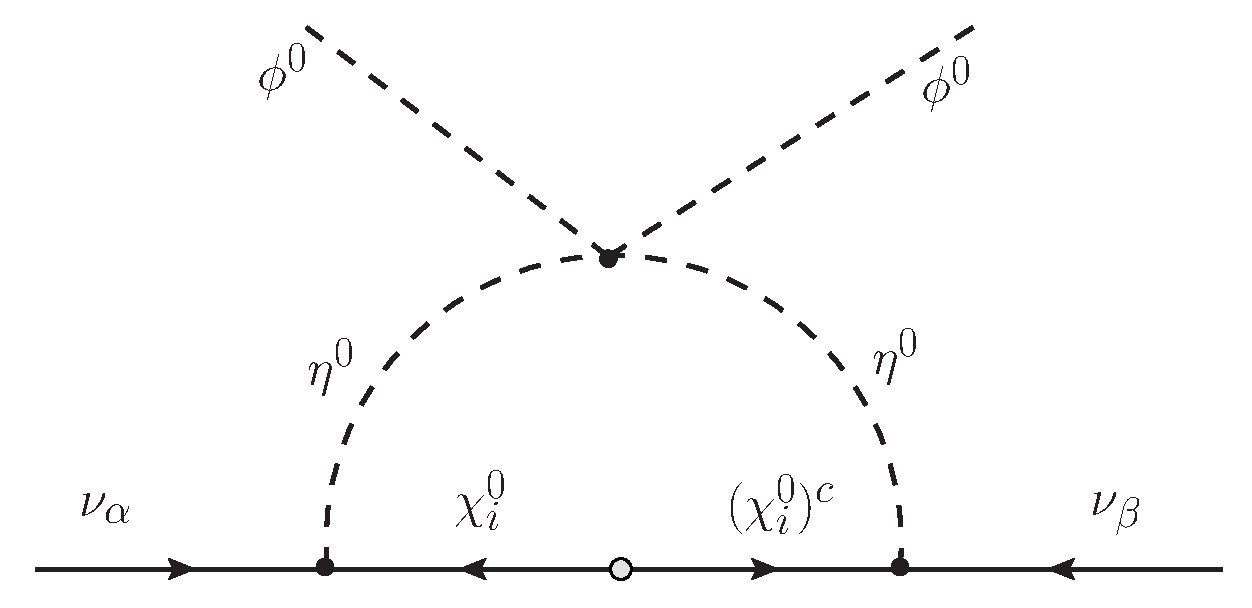
\includegraphics[scale=0.4]{mass-diagram}
\caption{1-loop diagram that generate masses in this model. }
\label{fig:mass-diagram}
\end{center}
\end{figure}
%
The neutrino mass matrix to 1-loop can be written as
%
\begin{align}
\label{eq:Mv-mass-matrix}
(\mathcal{M}_\nu)_{\alpha\beta} &= \sum_{i=1}^2\dfrac{h_{\alpha i}\,h_{\beta i}\,m_{\chi_i^0}}{2(4\pi)^2}
\left[
\dfrac{m_{\eta^R}^2\ln\left(\dfrac{m_{\chi_i^0}^2}{m_{\eta^R}^2}\right)}{m_{\chi_i^0}^2-m_{\eta^R}^2}
-\dfrac{m_{\eta^I}^2\ln\left(\dfrac{m_{\chi_i^0}^2}{m_{\eta^I}^2}\right)}{m_{\chi_i^0}^2-m_{\eta^I}^2}
\right] = \sum_{i=1}^2h_{\alpha i}\,\Lambda_i\,(h^T)_{i\beta}
=(h\,\Lambda\,h^T)_{\alpha\beta}\,,
\end{align}
%
where $h$ and $\Lambda$ are matrices, respectively given by
%
\begin{align}
\label{eq:h-Lambda-matrices}
h &= \dfrac{1}{\sqrt{2}}
\begin{pmatrix}
Y_{\Sigma}^1 & \sqrt{2}\,Y_N^1 \\
Y_{\Sigma}^2 & \sqrt{2}\,Y_N^2 \\
Y_{\Sigma}^3 & \sqrt{2}\,Y_N^3
\end{pmatrix}
\cdot V^{T}(\alpha)\,,
\hspace{1 cm}
\Lambda=
\begin{pmatrix}
\Lambda_1 & 0 \\
0 & \Lambda_2
\end{pmatrix}\,,
\end{align}
%
with
\begin{align}
\label{eq:Lambdai-definition}
\Lambda_i = \dfrac{m_{\chi_i^0}}{2(4\pi)^2}
\left[
\dfrac{m_{\eta^R}^2\ln\left(\dfrac{m_{\chi_i^0}^2}{m_{\eta^R}^2}\right)}{m_{\chi_i^0}^2-m_{\eta^R}^2}
-\dfrac{m_{\eta^I}^2\ln\left(\dfrac{m_{\chi_i^0}^2}{m_{\eta^I}^2}\right)}{m_{\chi_i^0}^2-m_{\eta^I}^2}
\right] \,.
\end{align}
%
Note that in the limit of $m_{\eta^R}= m_{\eta^I}$ we have a zero neutrino masses. This vanishing can can be understood because according with the eq.~\ref{eq:masa-etaR} and~\ref{eq:masa-etapI} it means that $\lambda_5$=0 and therefore it can be impose a conserved lepton number in this model. Even more, it can be shown that in the limit where the $\chi_i^0$ eigenvalues are lighter that the other fields, we obtain a simple expression for the neutrino mass matrix in terms of $\lambda_5$~\cite{Hirsch:2013ola}, it is
%
\begin{align}
\label{eq:Mv-aproximations}
(\mathcal{M}_\nu)_{\alpha\beta} &\approx \sum_{i=1}^2\dfrac{h_{\alpha i}\,h_{\beta i}}{(4\pi)^2}
\dfrac{\lambda_5 v_{\phi}^2}{m_0^2}
m_{\chi_i^0}\,,
\end{align}  
%
where 
\begin{align}
\label{ec_mo-definition}
m_0^2 = m_{\eta}^2 + \dfrac{1}{2}\left(\lambda_3+\lambda_4\right) v_{\phi}^2
+ \dfrac{1}{2}\lambda^{\eta}v_{\Omega}^2 - \dfrac{1}{\sqrt{2}}v_{\Omega}\,\mu_2\;
 \Rightarrow \;
 m_{\eta^{I,R}}^2 =m_0^2\pm\lambda_5 v_{\phi}^2\,.
\end{align}
%
It is convenient express the Yukawas couplings $h_{\alpha i}$ in the eq.~\ref{eq:Mv-mass-matrix} using the Casas-Ibarra parametrization~\cite{Casas:2001sr, Ibarra:2003up}. It turns out that
%
\begin{align}
h = U^*\sqrt{\widetilde{M}}\,R\,\sqrt{\Lambda}^{-1}\,, 
\end{align}
%
where $U$ is the PMNS (Pontecorvo-Maki-Nakagawa-Sakata) matrix, $\widetilde{M}=\text{diag}(m_1,m_2,m_3)$ with $m_i$ the neutrino physical masses, $\Lambda$ is given by the eq.~\ref{eq:h-Lambda-matrices} and $R$ is a $3\times 2$ complex, arbitrary and orthogonal matrix, such that $R\,R^T=\mathbb{I}_{3\times3}$. The $R$ matrix is similar to that one found in the context of type-one seesaw wit two generations of right-handed neutrinos, where we obtain one massles neutrino~\cite{Ibarra:2003up}. It depends of the neutrino hierarchy (NH: Normal hierarchy, IH: Inverse hierarchy),
%
\begin{align}
\label{eq:R-matrix}
R=\begin{pmatrix}
0 & 0 \\
\cos\gamma & \sin\gamma \\
-\sin\gamma & \cos\gamma
\end{pmatrix}\hspace{0.5 cm} &\text{for NH}\,,&\hspace{1.0 cm}
R=\begin{pmatrix}
\cos\gamma & \sin\gamma \\
-\sin\gamma & \cos\gamma \\
0 & 0
\end{pmatrix}\hspace{0.5 cm} &\text{for IH}& \nonumber \\
&m_1 \rightarrow 0&   &m_3 \rightarrow 0\,,& 
\end{align}
%
where $\gamma$ is in general a complex angle.














%%%++++++++++++++++++++++++++++++++++++++++++++++++++++++++++++++++++++++++++++++
\section{The compatibility between the dark matter and neutrino physics}
\label{sec:full-scan}

In order to study the DM phenomenology of this model, we scan the parameter space by considering the ranges that are shown in Table~\ref{tab:scan-parameter}. We fixed $m_{\eta}$ and $M_{\Sigma} > 100$ GeV in order to be conservative with LEP searches of charge particles~\cite{ALEPH:2005ab} and $v_{\Omega}<5$ GeV constrained by the $W$ gauge boson mass~\cite{Agashe:2014kda}. 
The remaining parameters were compute from this set. In particular, $m_{\Omega}$ was compute using the tadpole eq.~\ref{eq:tadpole-Omega}, $\lambda_1^{\text{SM}}$ and $m_{\phi}^2$ in the scalar potential~\ref{eq:scalar-potential} were fixed by the tadpole eq.~\ref{eq:tadpole-phi} and the mass for the scalar of the standard model, $m_{h}\approx 125$ GeV.
%
\begin{table}
\centering
\begin{tabular}{|c|c|}
\hline
Parameter & Range\\
\hline
$M_N$ &  $1-10^4$ (GeV) \\
$M_{\Sigma}$ &  $100-10^4$ (GeV) \\
$m_{\eta}$ &  $100-10^4$ (GeV) \\
$\mu_i$ & $1-10^{5}$ (GeV) \\
$|\lambda_i|$ , $|\lambda_i^{\Omega}|$ , $|\lambda^{\eta}|$ & $10^{-4} - 1$ \\
$v_{\Omega}$ & $10^{-2}- 5$  (GeV)\\
\hline
\end{tabular}
\caption{Scanning parameter ranges.}
\label{tab:scan-parameter}
\end{table}
%
We did  a carefully ramdom search where we imposed the theoretical constraints given by the eq.~\ref{eq:co-positivity} and the correct Yukawa coupling $Y_{\Sigma}^i$, $Y_N^i$ that reproduced the neutrino oscillation parameters~\cite{Forero:2014bxa, deSalas:2017kay}. In order to do that, we follow the algorithm described in sec.~\ref{sec:neutrino-masses}\footnote{We realized that neutrino hierarchy (IH, NH) does not play an important role in the analysis, for that reason we select randomly both hierarchies.}.
%
After that, we implement this model in~\texttt{SARAH}~\cite{Staub:2008uz,Staub:2009bi,Staub:2010jh,Staub:2012pb,Staub:2013tta} couple to the \texttt{SPheno}~\cite{Porod:2003um,Porod:2011nf} routines. 
Later, we used~\texttt{MicrOMEGAs 4.2.5}~\cite{Belanger:2006is} in order to compute the relic density and we only took the models that fulfill the current value $\Omega h^2 = (0.120 \pm 0.001)\; \text{to}\; 3\sigma$~\cite{Aghanim:2018eyx}.
We realized, although the mixture between the triplet fermion $\Sigma^0$ and the singlet fermion $N$ is important, the parameters space that is full consistent with the DM framework and the neutrino physics status, prefers a singlet component. 
In the left plot of Fig.~\ref{fig:MN-and-MTF} we show that the mass of the DM particle is principally the mass of the singlet fermion $M_N$. Even more, in the right plot of this figure, we can see that the difference between the mass of the DM particle and the triplet fermion mass $M_{\Sigma}$. 
We realized that $|m_{\chi^0} -m_{\Sigma}|$ is always bigger than $10$ GeV  for $m_{\chi^0}<2\times 10^3$ GeV and for $m_{\chi^0} >2\times 10^3$ GeV the model recovers the known limit of the Minimal DM scenarios when the DM particle is the triplet $\Sigma$ and the co-annihilation process are important. 
In those plots we show in color the quantity
%
\begin{align}
\label{eq:xi}
\xi &=\dfrac{|M_\Sigma - m_{\chi^0}|}{m_{\chi^0}}
\end{align}
%
that was introduce in~\cite{Hirsch:2013ola} as a indicator of the behavior of the singlet-triplet mixing in all the full region.
%
\begin{figure}
\begin{center}
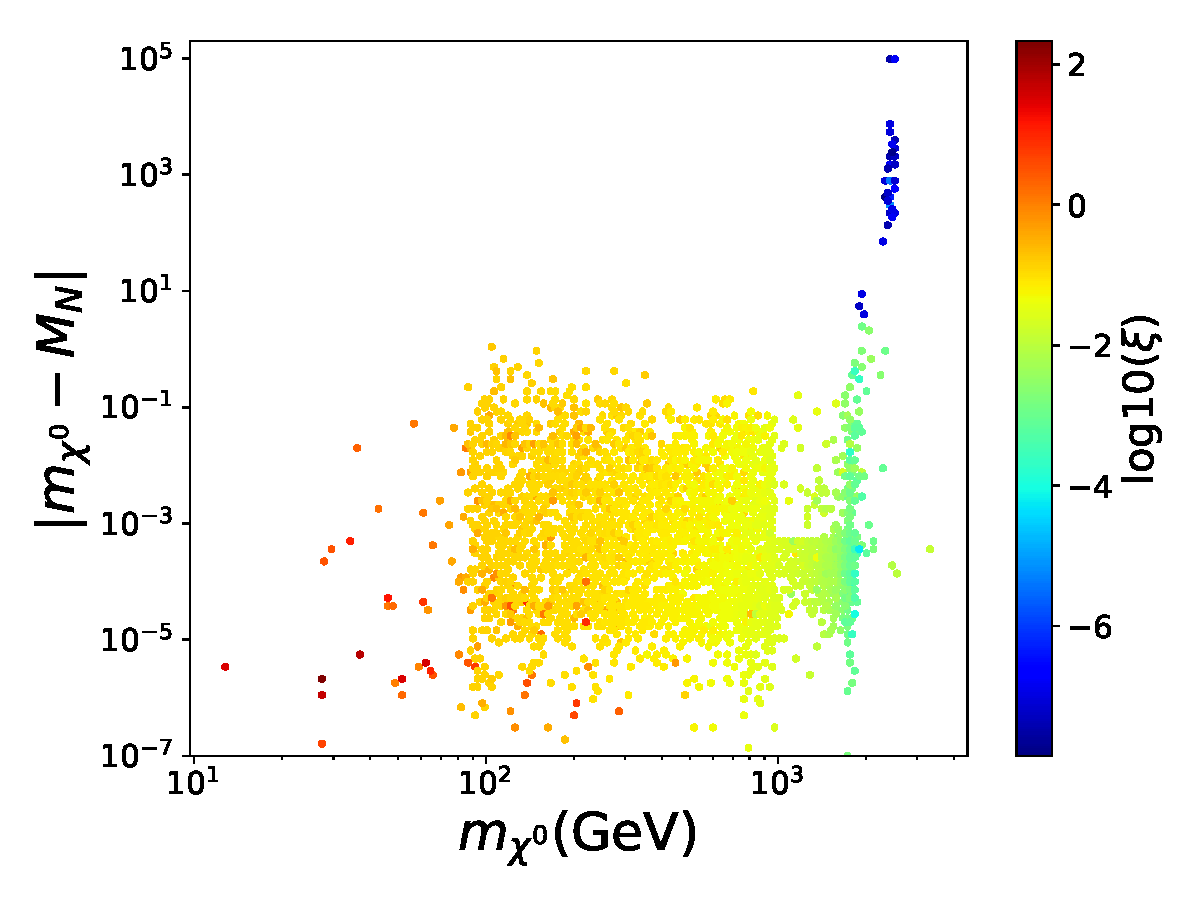
\includegraphics[scale=0.43]{mxoMN_with_neutrino_physics}
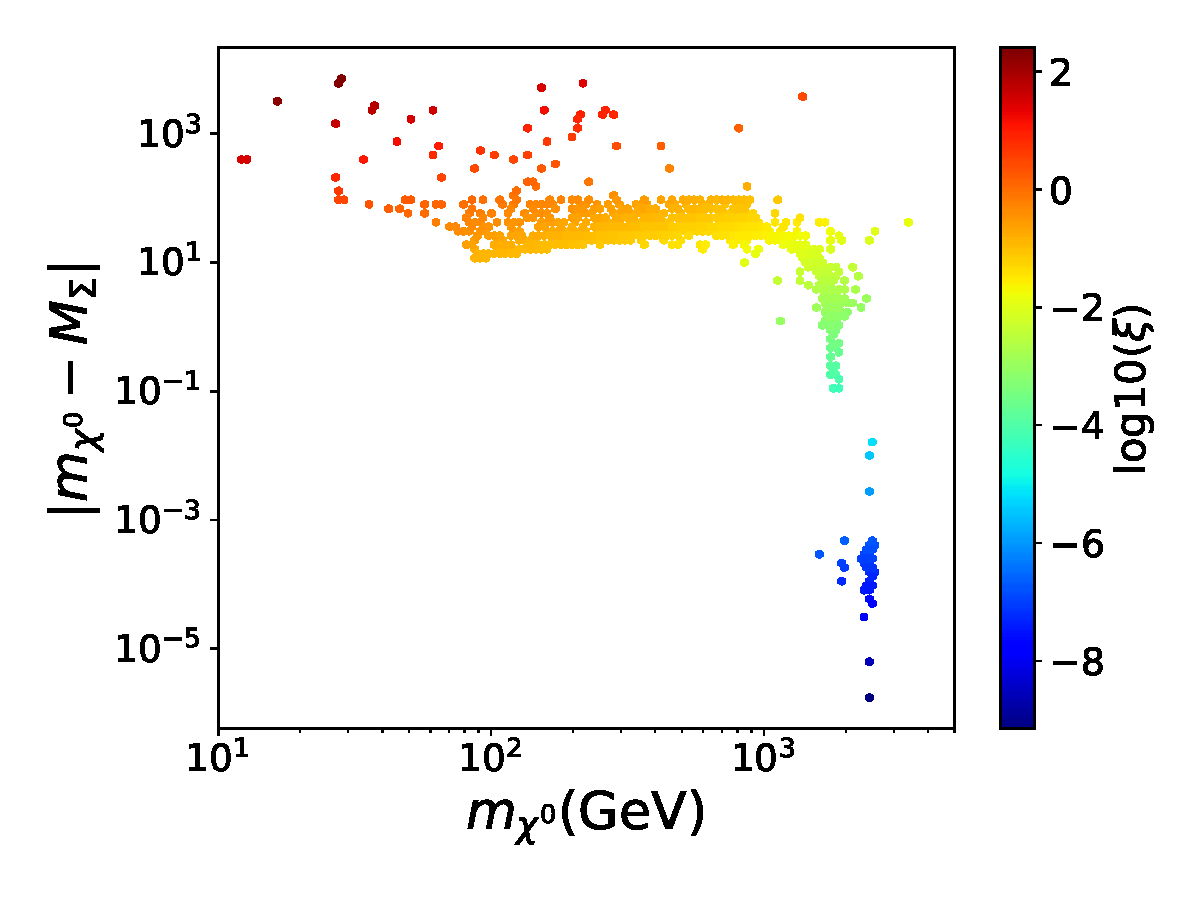
\includegraphics[scale=0.43]{mxoMTF_with_neutrino_physics}
\caption{Parameter space that is fully consistent with DM and neutrino physics in the singlet-triplet scotogenic model. In color, we show the variable $\xi$ define in the eq.~\ref{eq:xi}. Biggers values of $\xi$ is the limit for singlet fermion model $\sim N$ and shorts values correspond to the limit for triplet fermion DM $\sim \Sigma^0$.}
\label{fig:MN-and-MTF}
\end{center}
\end{figure}
%







\subsection{The status of direct-indirect detection of dark matter }
\label{sec:indirect-direct-detection}
A tree level, this model produce direct detection signal. In particular, it has nuclear recoils, i.e., it has an SI cross-section ($\sigma_{SI}$) and it is blind to SD signals because we do not have a tree level coupling between the DM and $Z$ gauge boson. 
%
\begin{figure}
\begin{center}
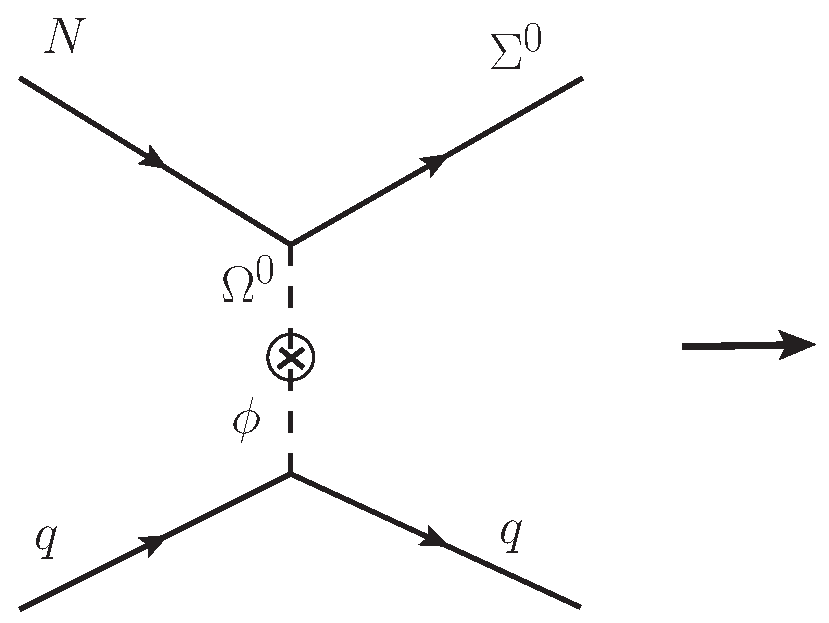
\includegraphics[scale=0.35]{SI}
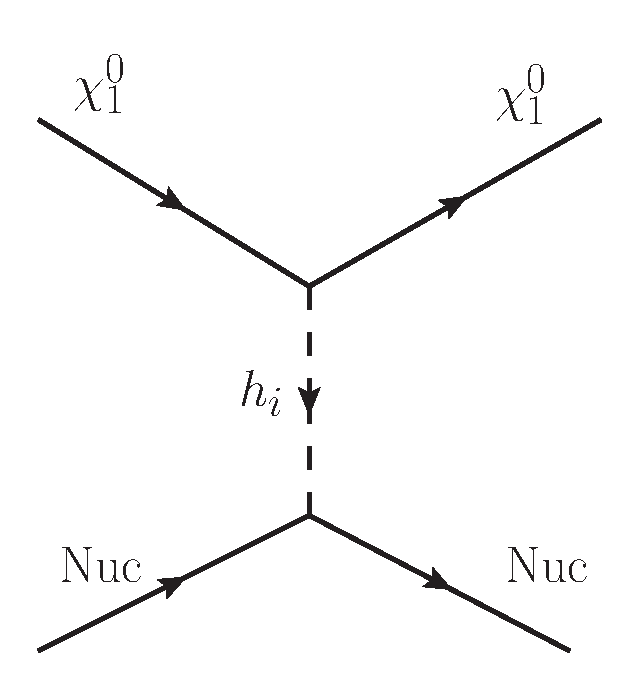
\includegraphics[scale=0.35]{SI-mass-basis}
\caption{SI process in the singlet-triple scotogenic model. In the left, we show the process in the guage basis. In the in right, we show the process in the mass basis in order to show that actually we have to contributions coming from the two higgses $h_i$.}
\label{fig:SI-diagram}
\end{center}
\end{figure}
%
The SI scattering process between the DM an the nucleon are mediated by the two higgses $h_i$ of the model that comes from the mixing between the scalars $\Omega^0$ and $\phi$. The process is shown in Fig.~\ref{fig:SI-diagram} and it is easily computed, in the limit where the  Mandelstam variable $t$ is negligible. It is given by
%
\begin{align}
\label{eq:sigma-SI}
\sigma_{SI}=\dfrac{\mu_{\text{red}}^2}{\pi}\left[\dfrac{M_{\text{Nuc}}f_N}{v}\dfrac{Y_{\Omega}\sin(2\alpha)\sin(2\beta)}{2}\left(\frac{1}{m_{h_2}^2}-\frac{1}{m_{h_1}^2}\right)\right]^2\,,
\end{align}
%
where, $M_{\text{Nuc}}$ is the nucleon mass, $f_N\approx 0.3$ is the nucleon form factor, $\mu_{\text{red}}= m_{\chi^0}M_{\text{Nuc}}/(m_{\chi^0}+M_{\text{Nuc}})$ is the reduced mass of the system and  $m_{h_i}$ is the mass of the higgs $h_i$.

\begin{figure}
\begin{center}
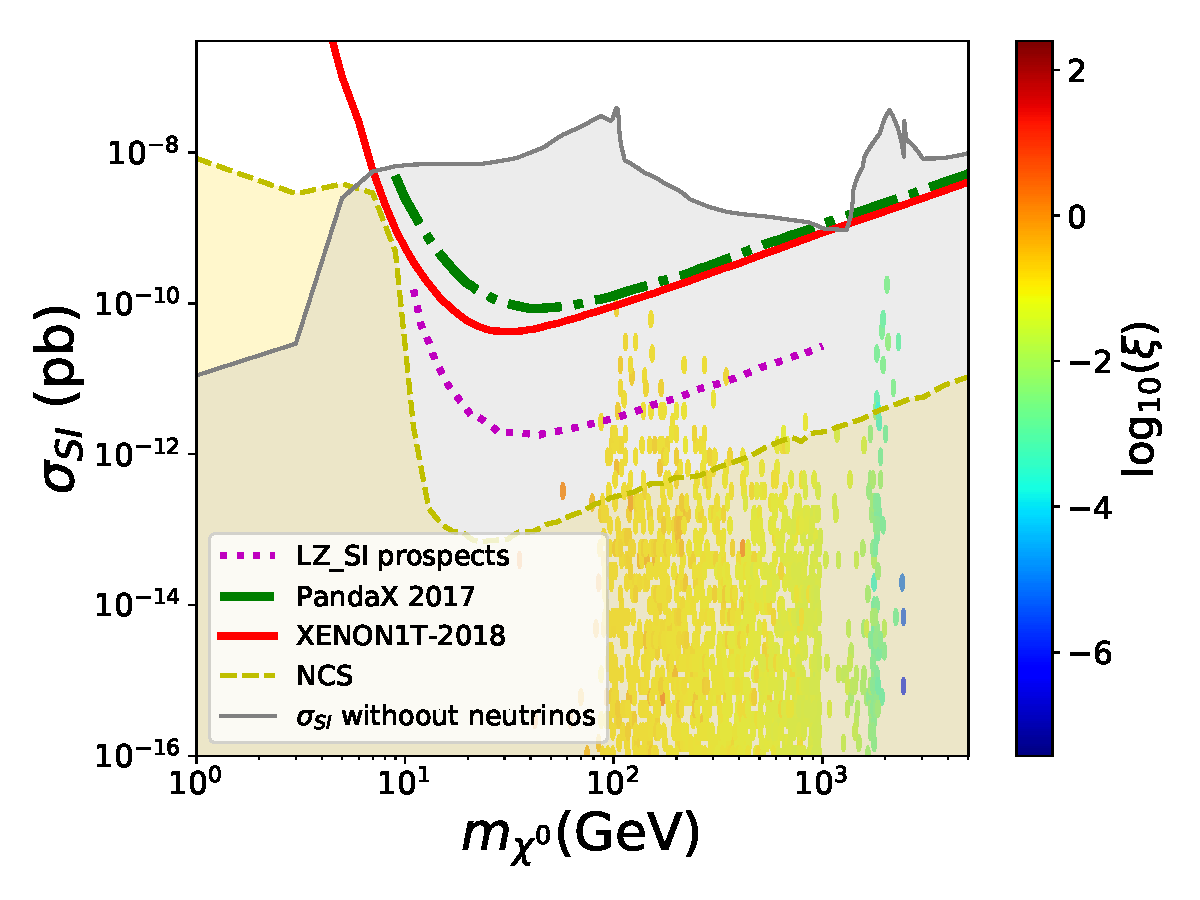
\includegraphics[scale=0.43]{sigmaSI_with_neutrino_physics}
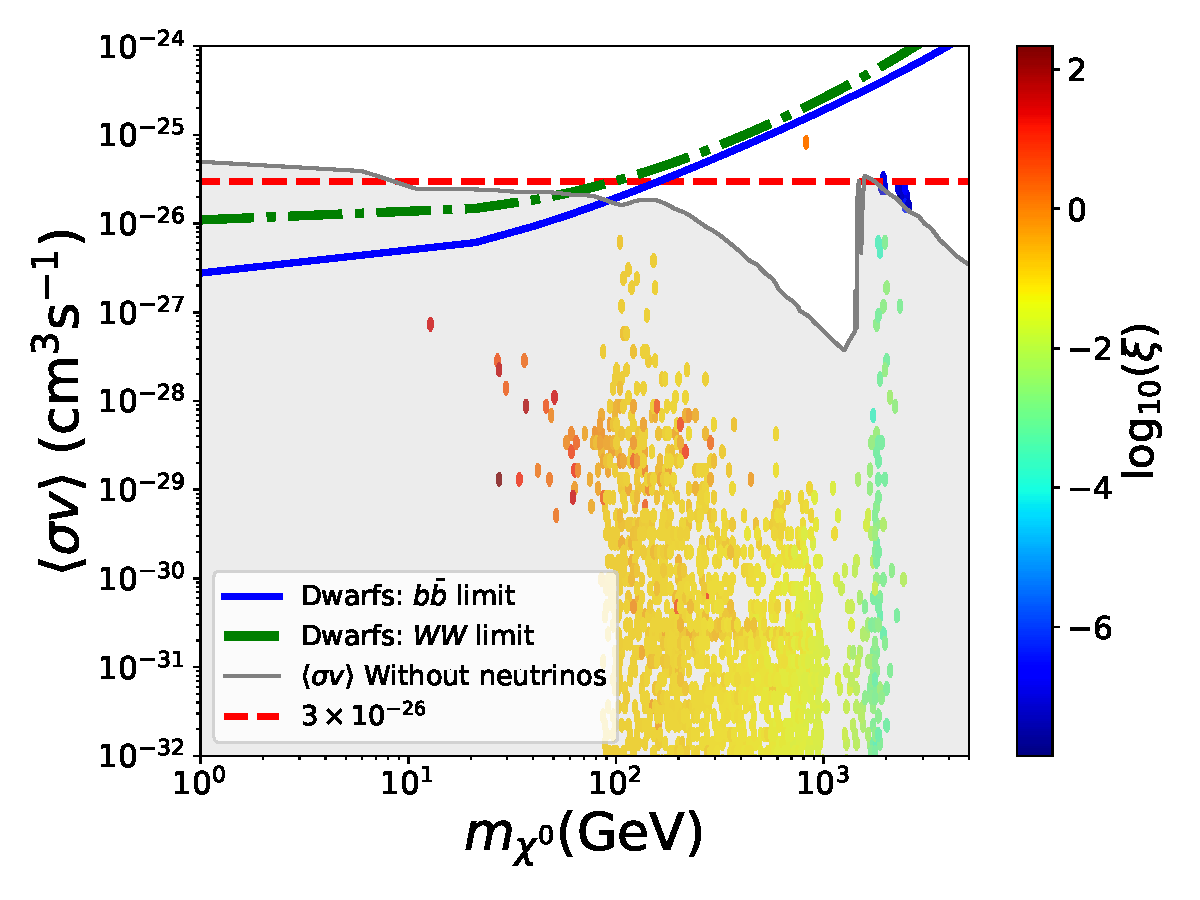
\includegraphics[scale=0.43]{sigmav_with_neutrino_physics}
\caption{Left: SI cross-section. We show the currrents limits of XENON1T~\cite{Aprile:2018dbl}, PANDAS~\cite{Cui:2017nnn}, the LZ prospects~\cite{Mount:2017qzi} and the Neutrino Coherent Scattering (NCS)~\cite{Cushman:2013zza, Billard:2013qya}. 
Right:  Velocity averaged annihilation cross-section as a function of the DM
mass in comparison to current indirect detection limits in different channels. The $95\%$ C.L gamma-ray upper limits from dSphs were extracted from ref.~\cite{Ackermann:2015zua}.
In both plots, we show  the region compatible with the relic density but without the correct Yukawas that reproduce the neutrino oscillation parameters. In colors, we plot the $\xi$ variable defined in the eq.~\ref{eq:xi}.
}
\label{fig:SI-and-sv-with-neutrinos-scan}
\end{center}
\end{figure}

We compute the $\sigma_{SI}$ for each point of the scan that was compatible with the relic density of the DM and the neutrino physics at the same time. Even more, we did a cross-check with the \texttt{MicrOMEGAs 4.2.5} rutine~\cite{Belanger:2006is}. 
Our results are shown in the left part of Fig.~\ref{fig:SI-and-sv-with-neutrinos-scan} with the current experimental limits of XENON1T~\cite{Aprile:2018dbl}, PANDAS~\cite{Cui:2017nnn} and the LZ prospects~\cite{Mount:2017qzi}. 
After this, we clearly see that the scan prefers the region with a DM mass $m_{\chi^0}\gtrsim 100$ GeV. 
Even more, we assure that the region with low DM mass will be excluded by LFV processes as we will show in the next section.
We can see that the model is no seriously restrige by the current experimental searches. Even more, the majority of the points fall into the Neutrino Coherent Scattering (NCS)~\cite{Cushman:2013zza, Billard:2013qya}, were they will be challenging to looking for in the future.
Perhaps, the most important feature is that the neutrino oscillation parameters drastically restring the parameter space of the model. 
After the Casas-Ibarra routine described section~\ref{sec:neutrino-masses}, the model gives us Yukawa couplings $Y_{\Sigma}^i$ and $Y_N^i$ all of them in the range $1^{-4}<|Y_{\Sigma, N}^i|<1$. By construction, they reproduce the neutrino phyiscs and they reduced drastically the parameter space of the model. In order to show that, we plot in grey the contour of the naked parameter space that is only compatible with DM and was established in the ref.~\cite{Hirsch:2013ola}.   

On the other hand, we used the \texttt{MicrOMEGAs 4.2.5} routine~\cite{Belanger:2006is} to compute the velocity annihilation cross-section $\langle \sigma v\rangle$ of this model for each point of the scan that was compatible with the relic density of the DM and the neutrino physics at the same time. 
It is shown in the right part of Fig.~\ref{fig:SI-and-sv-with-neutrinos-scan} with the $95\%$ C.L gamma-ray upper limits from dSphs for DM annihilation into $b\bar{b}$ and $WW$~\cite{Ackermann:2015zua}.
As in the previous analysis, the region of low DM mas is seriously constrained by the neutrino physics. In grey, we plot the contour of the naked parameter space that is only compatible with DM and was established in the ref.~\cite{Hirsch:2013ola}.












%%%++++++++++++++++++++++++++++++++++++++++++++++++++++++++++++++++++++++++++++++
\section{Lepton Flavor Violation (LFV) processes}
\label{sec:LFV}

In this model we have LFV processes that seriously constrained its parameter space. Recently was shown that the most promising experiments perspectives are bases on $\mu\rightarrow 3 e$, $\mu - e$ conversion in nuclei and 3-body decays $l_{\beta}\rightarrow l_{\alpha}\gamma$ which $\mu\rightarrow e\gamma$ is the most important one~\cite{Rocha-Moran:2016enp}. 

Before doing this analysis we take care our previous findings. In sec.~\ref{sec:indirect-direct-detection} we realized that the mixing between the triplet $\Sigma^0$ and the singlet $N$ is necessary in order to get the correct relic density of the DM with a fermion mass $m_{\chi^0} < 2.7$ TeV. However, we found that in the special region with $100\; \text{GeV} < m_{\chi^0} < 1$ TeV, the eigenvalue given by the mixing is almost singlet. This was assure by the value of the $\xi$ parameters plotted in all previous figures. 
Even more, we checked that mixed angle defined by the eq.~\ref{eq:M-chi-rotation} fulfill that $\cos\alpha\approx 0$ and $\sin\alpha\approx 1$ in this region. 
%
\begin{figure}
\begin{center}
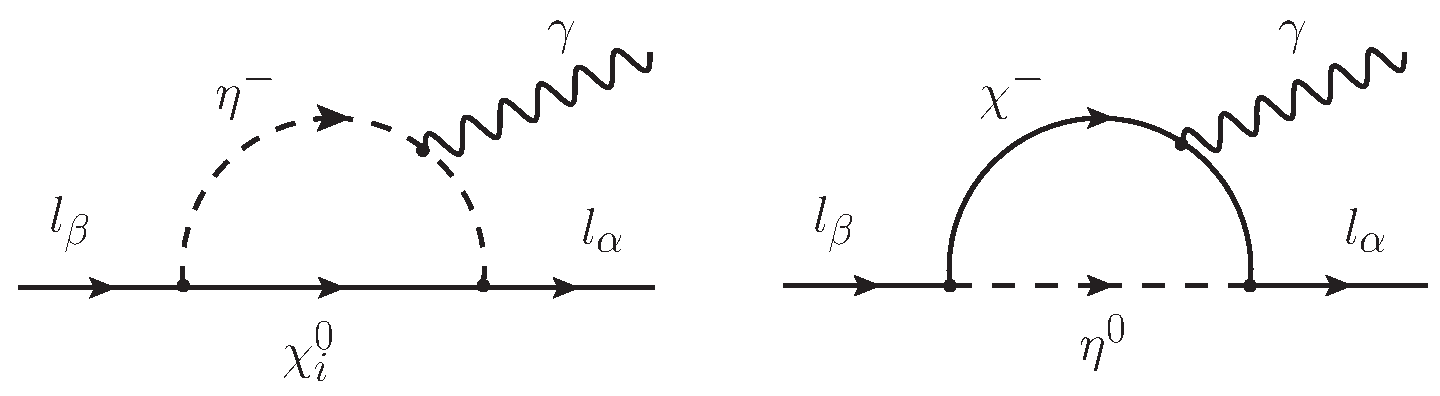
\includegraphics[scale=0.55]{LFV-diagrams}
\caption{Dominant Feynman diagrams in the $l_{\beta}\rightarrow l_{\alpha}\gamma$ process.}
\label{fig:mu-e-gamma}
\end{center}
\end{figure}
%
Therefore, we computed the $l_{\beta}\rightarrow l_{\alpha}\gamma$ process in this limit.
Its principal contributions comes from the Feynman diagrams shown in Fig.~\ref{fig:mu-e-gamma} which the left diagram with neutral fermion in the loop is common to the original scotogenic model~\cite{Toma:2013zsa,Ibarra:2016dlb}. However, the diagram with the charged fermion in the loop is characteristic of this model, i.e., we have two contributions. The former comes from the mixing of the neutral fermions and the last comes from the charge fermion $\Sigma^{\pm}$. The branching ratio for this process is approximately given by
%
\begin{align}
\label{eq:mu-e-gamma}
\text{Br}(l_{\beta}\rightarrow l_{\alpha}\gamma) &\approx
\dfrac{3\,\alpha_{em}\text{Br}(l_{\beta}\rightarrow l_{\alpha}\nu_{\beta}\bar{\nu}_{\alpha})}{64\,\pi G_F^2 } \nonumber \\
&\left|\dfrac{Y_{N\alpha}Y_{N\beta}^* F_2\left(\xi_1\right)
+\dfrac{1}{2}Y_{\Sigma\alpha}Y_{\Sigma\beta}^* F_2\left(\xi_2\right)
}{m_{\eta^{\pm}}^2}
-\dfrac{1}{m_{\eta^{0}}^2}Y_{\Sigma\alpha}Y_{\Sigma\beta}^* G_2\left(\dfrac{m_{\chi^{\pm}_2}^2}{m_{\eta^{0}}^2}\right)
\right|^2 \,,
\end{align}
%
where,
%
\begin{equation}
\xi_i=\dfrac{ m_{\chi_i^0}^2 }{  m_{\eta^{\pm}}^2 }
\end{equation}
%
%\begin{equation}
%\rho = \dfrac{ m_{\chi_i^{\pm}}^{2} }{  m_{\eta^{0}}^2 }
%\end{equation}
%
\begin{equation}
\label{eq:F2}
F_2(z)=\dfrac{1-6z+3z^2+2z^3-6z^2\ln{z}}{6(1-z)^4}
\end{equation}
%
\begin{equation}
\label{eq:G2}
G_2(z)=\dfrac{2+3z-6z^2+z^3+6z\ln{z}}{6(1-z)^4}\,.
\end{equation}
%
We clearly see the two contribution of the diagrams shown in Fig.~\ref{fig:mu-e-gamma}. Even more, we check that in the limit of the single scotogenic model, we recover the expression reported in the ref.~\cite{Ibarra:2016dlb} and in the limit of $\cos\alpha\approx 0$ we recover the expression reported in the ref.~\cite{Rocha-Moran:2016enp}.
%
\begin{figure}
\begin{center}
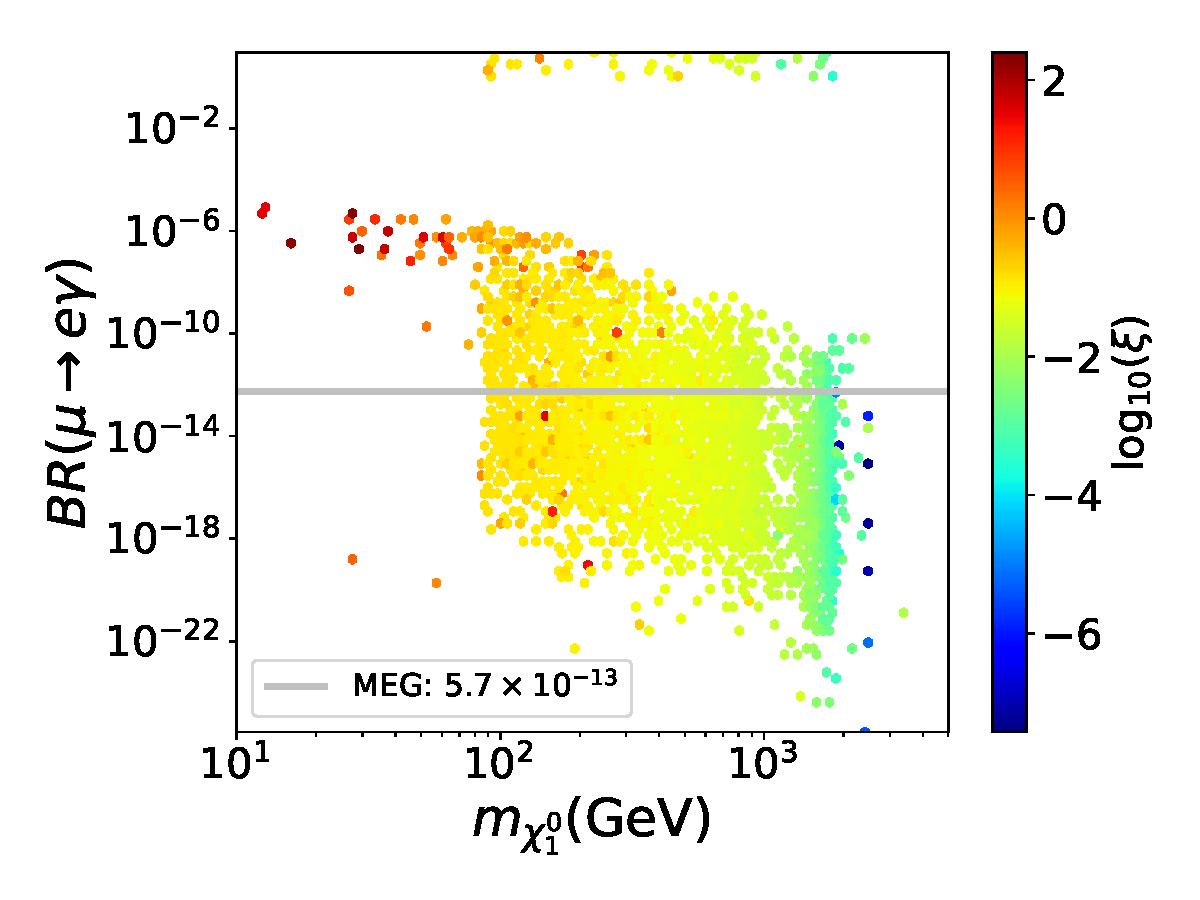
\includegraphics[scale=0.43]{ueg_with_neutrino_physics}
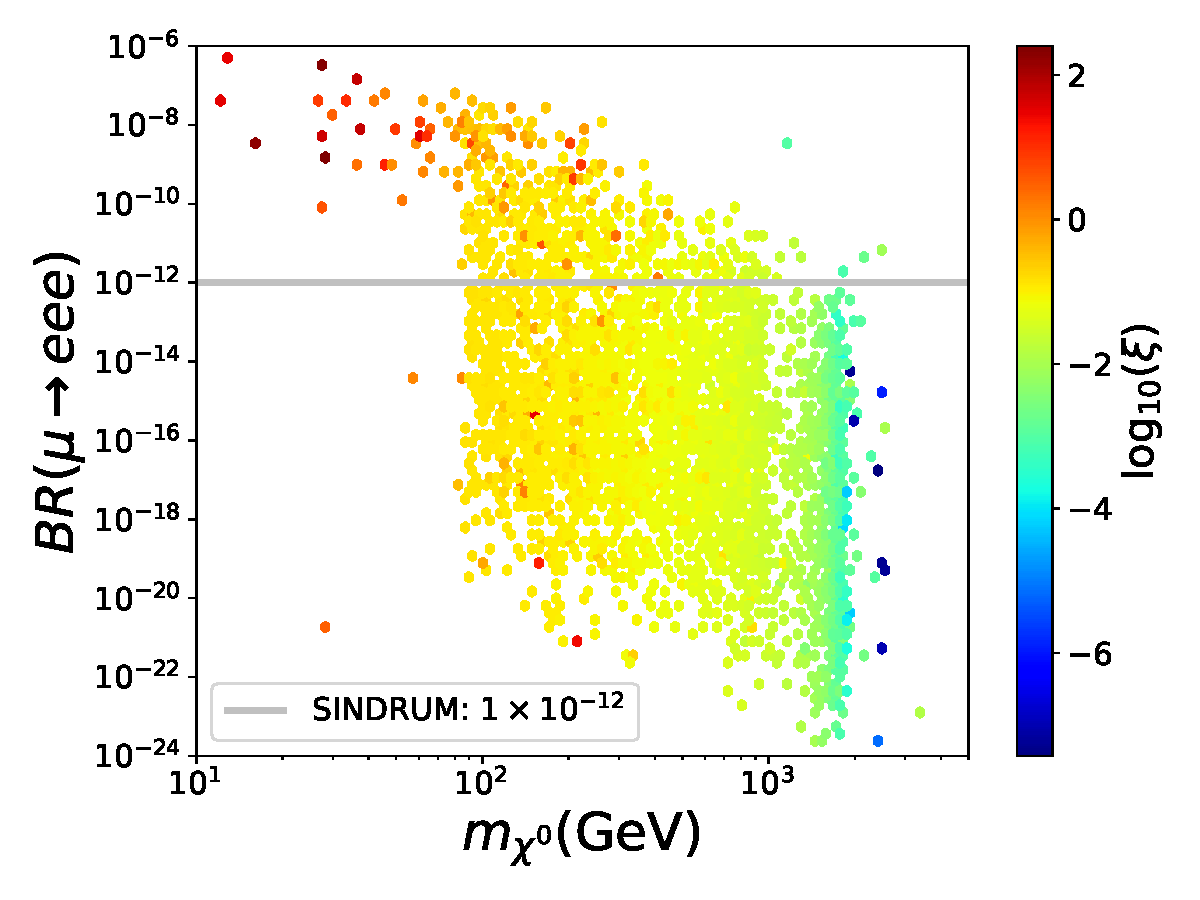
\includegraphics[scale=0.43]{u3e_with_neutrino_physics}
\caption{Left: $\mu\rightarrow e\gamma$ values for the scan of the parameter space agree with DM and the neutrino oscillation parameter. The grey line show the current limit~\cite{Adam:2013mnn}, i.e., the upper region is exclude.
Right: $\mu\rightarrow 3\,e$ values for the scan. The grey line show the current limit~~\cite{Bertl:1985mw}.}
\label{fig:ueg-e3e}
\end{center}
\end{figure}
%
In the left part of Fig.~\ref{fig:ueg-e3e} we show the the behavior of the $\mu\rightarrow e\gamma$ process for the scan done in the previous section. Our analytical expression was checked with the \texttt{FalvorKit}~\cite{Porod:2014xia} of \texttt{SARAH}~\cite{Staub:2008uz,Staub:2009bi,Staub:2010jh,Staub:2012pb,Staub:2013tta} couple to the \texttt{SPheno}~\cite{Porod:2003um,Porod:2011nf} routines. Also, we show the current experimental bounds carry out by MEG experiment~\cite{Adam:2013mnn}. 
Even more, we compute numerically the $\mu\rightarrow 3\,e$ process which is shown in the right part of Fig.~\ref{fig:ueg-e3e} with its present bound given by the SINDRUM experiment~\cite{Bertl:1985mw}.
We realize that some points of the parameter space are excluded, specially those with bigger $\xi$ values. Even more, we can see that although LFV processes exclude almost all the region with $m_{\chi^0}\lesssim 100$ GeV, the majority of the models with $m_{\chi^0} \gtrsim 100$ GeV survives and the previous analysis does not change significantly. 

As a final part of this section, in Fig.~\ref{fig:model-parameters} we show the behavior of some of the parameters of the model that past all the last constraints
%
\begin{figure}
\begin{center}
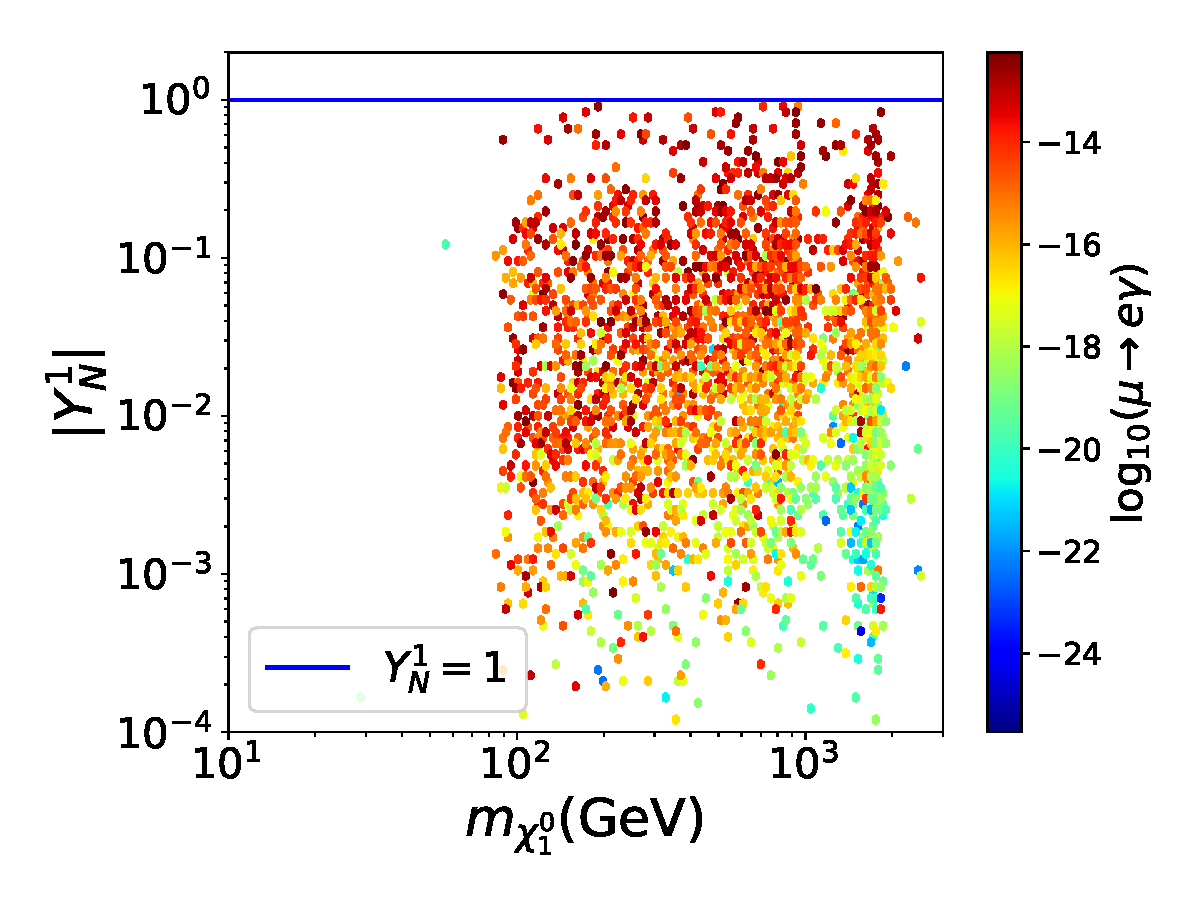
\includegraphics[scale=0.4]{YN1}
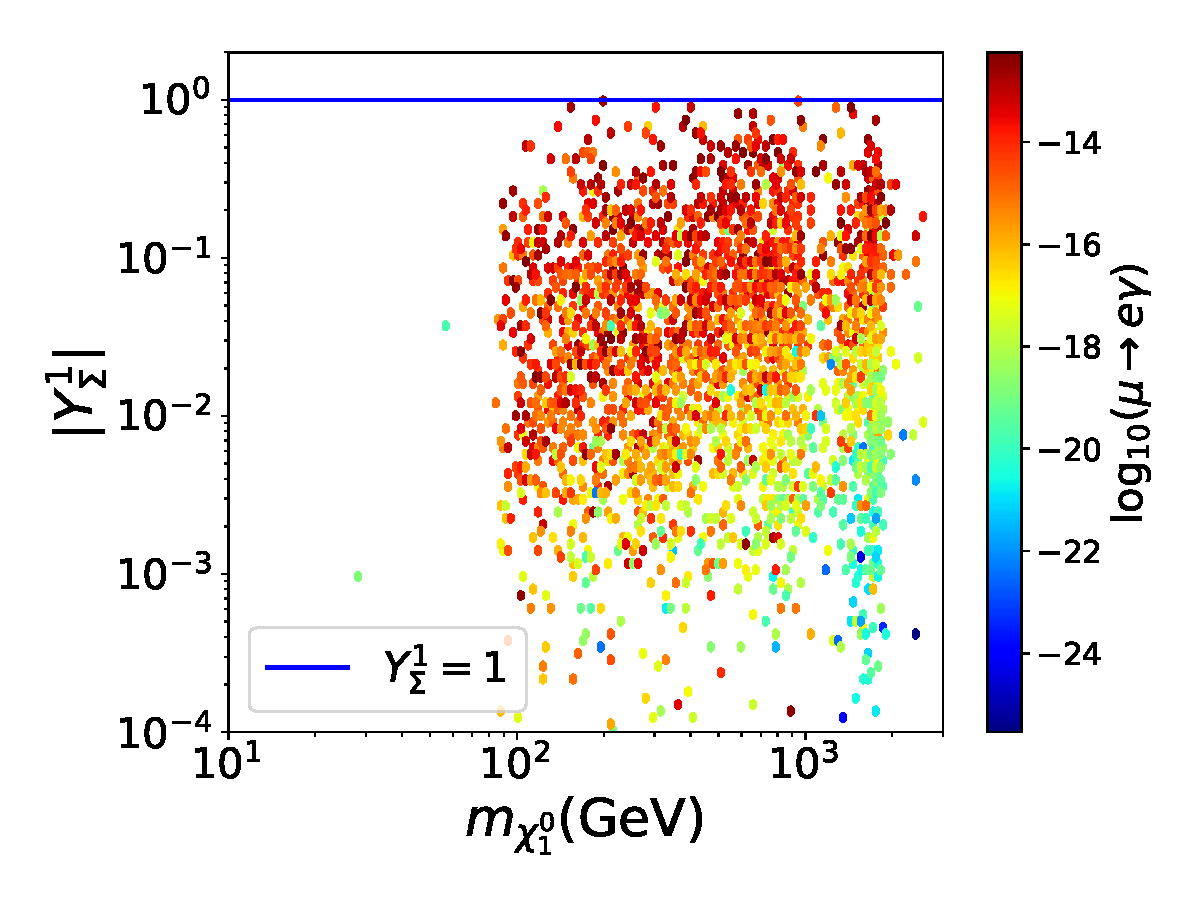
\includegraphics[scale=0.4]{YTF1}
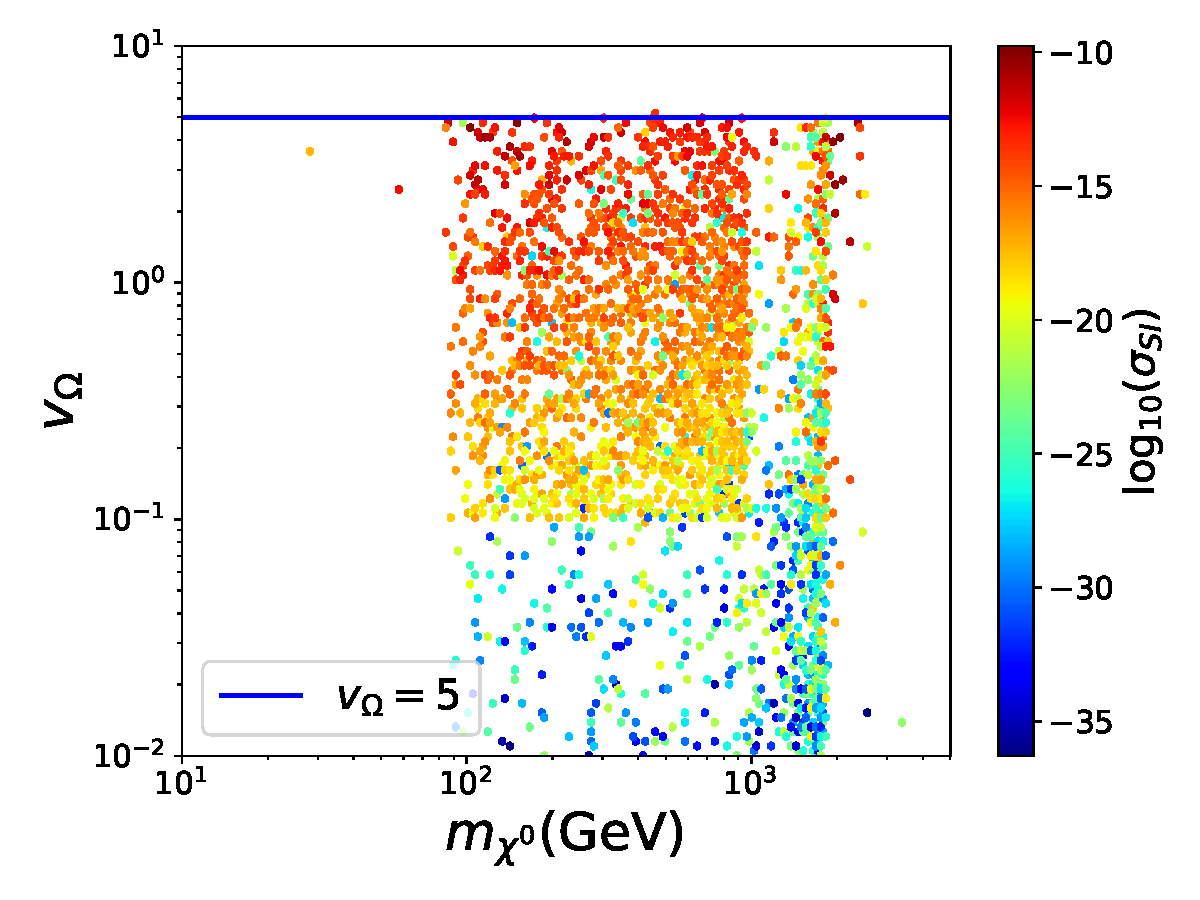
\includegraphics[scale=0.4]{vT}
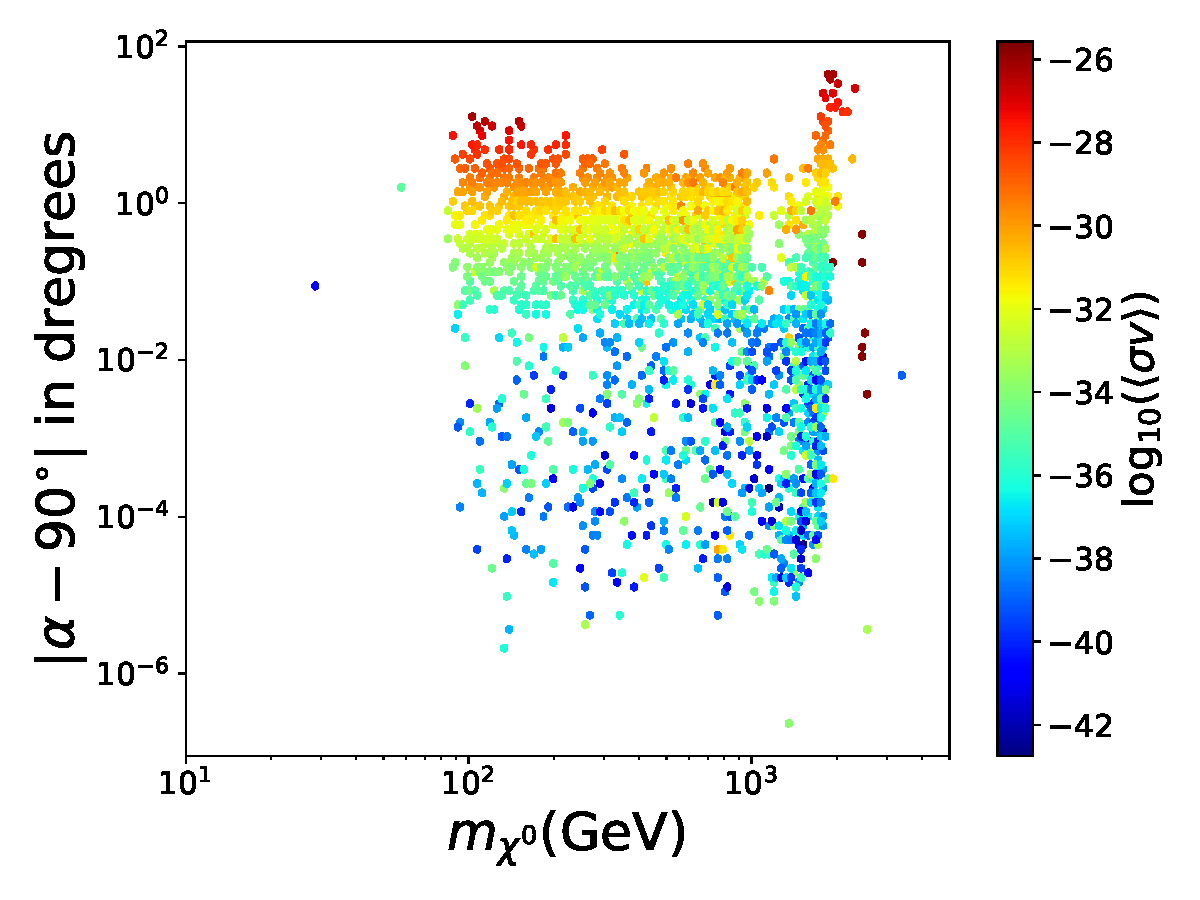
\includegraphics[scale=0.4]{alpha}
\caption{Behavior of the parameters of the singlet-triplet scotogenic model that fulfill DM, neutrino physics and LFV process.}
\label{fig:model-parameters}
\end{center}
\end{figure}
%
According with those plots we conclude the next features. The Yukawa couplings $Y_{N}^1$ and $Y_{\Sigma}^1$ control the $\mu\rightarrow e\,\gamma$ process. Bigger couplings than one give us LFV in this model as we show in the up plots of the figure with similar behavior is found for all the Yukawa couplings $Y_{N}^i$ and $Y_{\Sigma}^i$.
The VEV $v_{\Omega}$ of the triplet scalar controls the SI cross section as we expect by the construction of the model. 
The velocity averaged annihilation cross-section is clearly controlled by the mixing angle $\alpha$ defined in the ec.~\ref{eq:M-chi-rotation}. 
Sizable values for $|\alpha-90^{\circ}|$ give us sizable values for the $\langle\sigma v\rangle$ as we can see in lower-right part of this figure. Even more, we assure that those are the promising points that will create bigger fluxes of gamma-ray as we will see in next section.



 







%%%++++++++++++++++++++++++++++++++++++++++++++++++++++++++++++++++++++++++++++++
\section{1-loop prospect processes}
\label{sec:1-loop-processes}

In this section we compute some new observables to 1-loop level in this model that are forbidden to tree level. The former is the SD cross-section of DM recoil with nuclei and the last is DM annihilation into two photons. Both of them are promising process for future signals of this model.

\subsection{Spin-dependent cross-section to 1-loop}
\label{sec:sigma-SD}
%
\begin{figure}[h]
\begin{center}
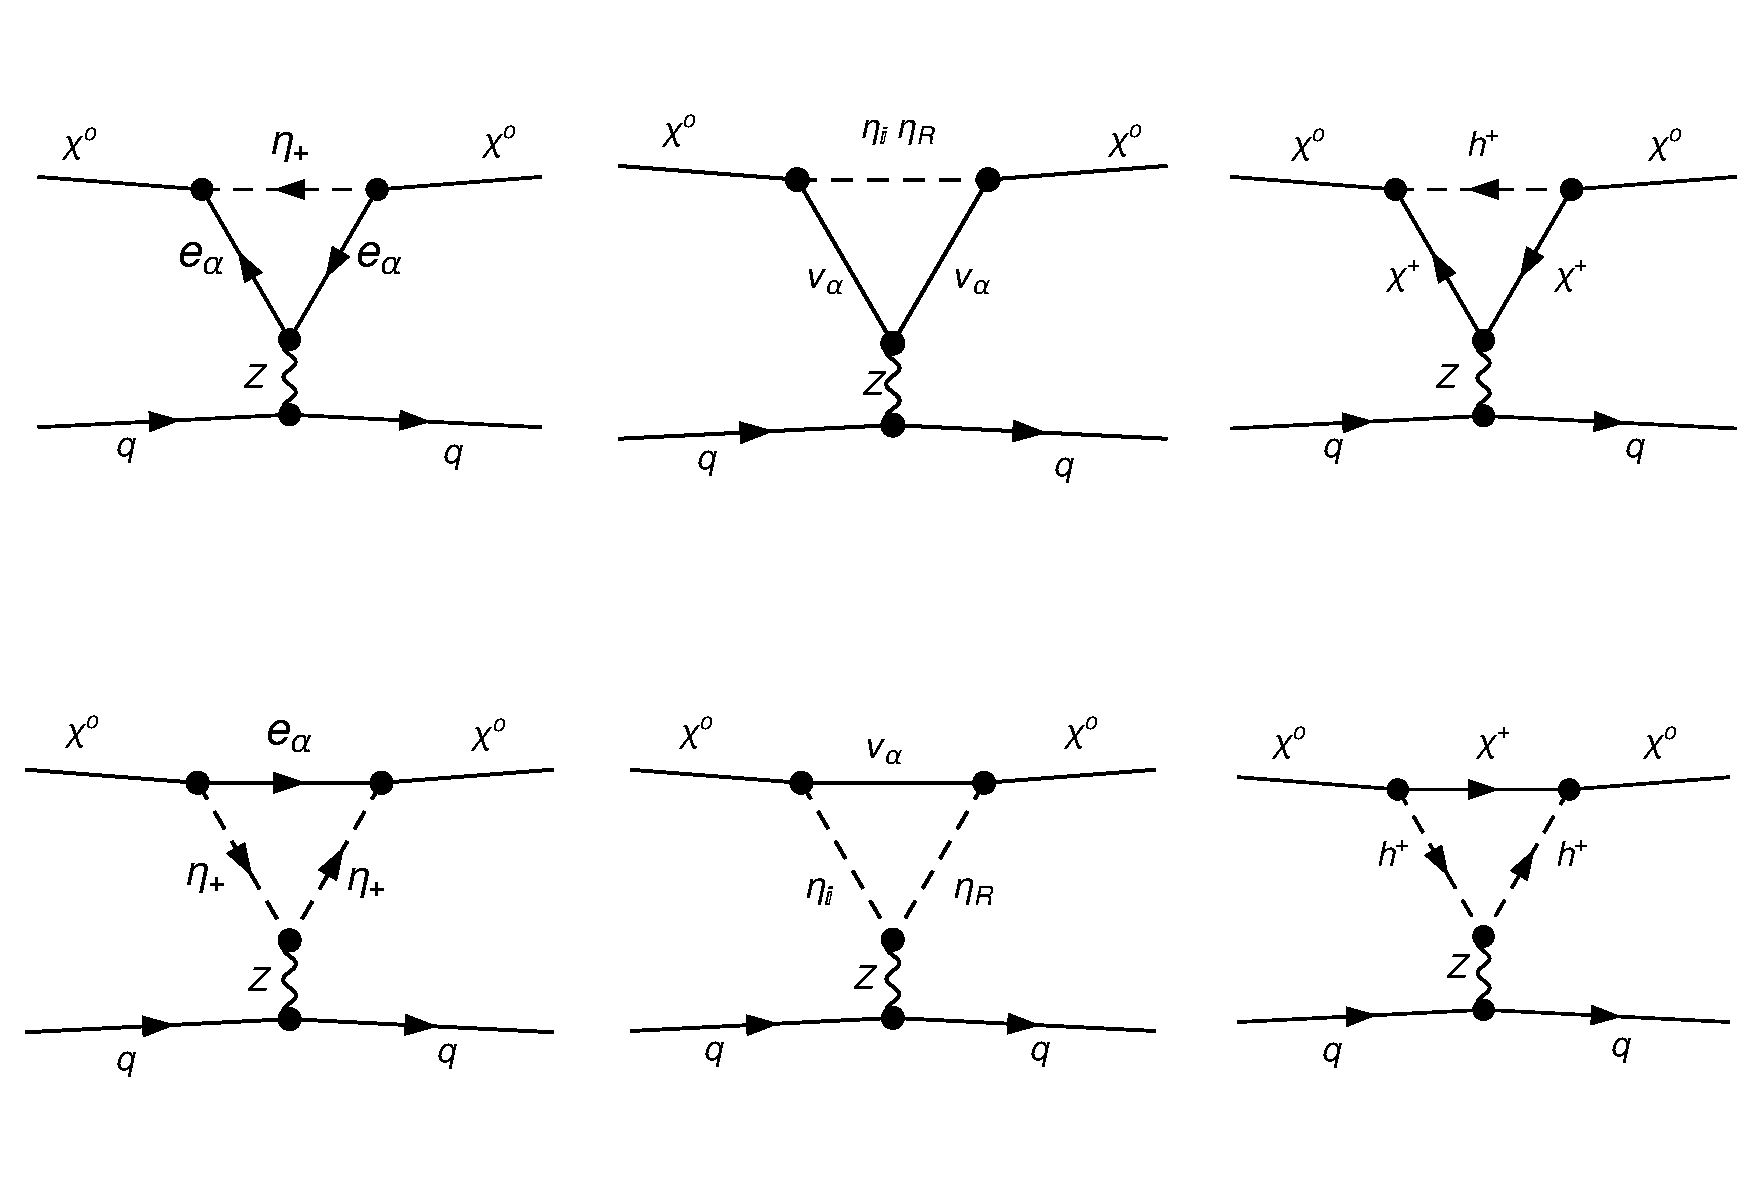
\includegraphics[scale=0.45]{SD-diagrams}
\caption{ Diagrams contributing to SD cross-section at 1-loop level. They were generated using \texttt{FeynArts}~\cite{Hahn:2000kx}. }
\label{fig:SD}
\end{center}
\end{figure}
%
Although this model is blind to SD scattering of DM at tree level, it can be generated at 1-loop level as is shown in Fig.~\ref{fig:SD}. Concretely,  the exchange of the  $Z$ gauge boson leads to an effective axial vector interaction term of the form~\cite{Jungman:1995df, Ibarra:2016dlb}
%
\begin{align}
\label{eq:LSD-eff}
\mathcal{L}_{\text{eff}}\, =\, \xi_q \bar{\chi^0}\gamma^{\mu}\gamma^5 \chi^0 \bar{q}\gamma_{\mu}\gamma^5q + \text{h.c.}\,,
\end{align}
%
where
%
\begin{align}
\label{eq:xiq}
\xi_q = \dfrac{a_q \sin^2\alpha }{32\pi^2M_Z^2}
\left\{
\sum_{\alpha}|Y_N^{\alpha} |^2\left[
(v_{e}+a_{e}) \mathcal{G}_2\left(\dfrac{m_{\chi^0}^2}{m_{\eta^{\pm}}^2}\right) 
+ (v_{\nu}+a_{\nu}) \mathcal{G}_2\left(\dfrac{m_{\chi^0}^2}{m_0^2}\right) 
\right]
+ 
Y_{\Omega}^2(v_{\chi}+a_{\chi}) \mathcal{G}_2\left(\dfrac{m_{\chi^0}^2}{m_{\Omega^0}^2}\right) 
\right\}\,,
\end{align}
%
with $a_q = \dfrac{1}{2} \left(-\dfrac{1}{2}\right)$ for $q=u,c,t\, (d,s,b)$, $a_{e} = -\dfrac{g}{2c_W}\left(\dfrac{1}{2}\right)$, $v_{e} = -\dfrac{g}{2c_W}\left(\dfrac{1}{2}-2s^2_W \right)$, $a_\nu = v_\nu = \dfrac{g}{2c_W}\left(\dfrac{1}{2}\right)$, $a_{\chi} = 0$, $v_{\chi} = -g\, c_W$, $m_{h^+}\approx m_{\Omega^0}$ and $ m_{\eta^R}\approx m_{\eta^I}=m_0$. $\mathcal{G}_2(z)$ is a loop function given by
%
\begin{align}
\label{eq:G2}
\mathcal{G}_2(z) = -1 + \dfrac{2(z+(1-z)\ln(1-z))}{z^2}\,.
\end{align}
%
The resulting SD cross-section per nucleon  $N$  is given by
%
\begin{equation}
\label{eq:SD}
\sigma_{SD}=\dfrac{16}{\pi}\dfrac{m_{\chi^0}^2m_N^2}{(m_{\chi^0}+m_N)^2}J_N(J_N+1)\left(\sum_{q=u,d,s}\Delta_q^N \xi_q\right)^2 \,,
\end{equation}
where $\Delta_u^N=0.842$, $\Delta_d^N= -0.427$ and $\Delta_s^N= -0.085$~\cite{Airapetian:2006vy}, $m_N$ is the nucleon mass and $J_N$ is the  total angular momentum of the nucleus. 
Notice that we have three contributions to the $\xi_q$ effective coupling. 
The first and the second are common to the original scotogenic model~\cite{Ma:2006km}, however, the third one with the fermion $\chi^{+}$ in the loop is characteristic of this model and could enhance the SD cross-section. Even more, we checked that in the limit of $\alpha\sim\pi/2$ and $Y_{\Omega}=0$ we recovered the results found in the ref.~\cite{Ibarra:2016dlb}.
In Fig.~\ref{fig:SD-scan} we show the behavior of the SD cross-section for all the models found in the previous section that generates the DM density via the freeze-out mechanism and saturate the value measured by the Planck satellite~\cite{Aghanim:2018eyx}. Also, those models generate the correct neutrino oscillation parameters~\cite{deSalas:2017kay} and are not excluded by the LFV process described in sec.~\ref{sec:LFV}. 
In this figure, we also show the IceCube~\cite{2013PhRvL.110m1302A} limits in the $W^+W^-$ channel (black solid line) from null observations of the sun, the limits from LUX~\cite{Akerib:2016lao} (yellow solid line) and the expected sensitivity of LZ and XENON1T experiments~\cite{Cushman:2013zza}(red(green) dashed(dot-dashed) line).
We realize that this model is not exclude by SD scattering of DM with nuclei, however, it could be proved in the future with the next generation of experiments as LZ and XENON1T.
%
\begin{figure}[h]
\begin{center}
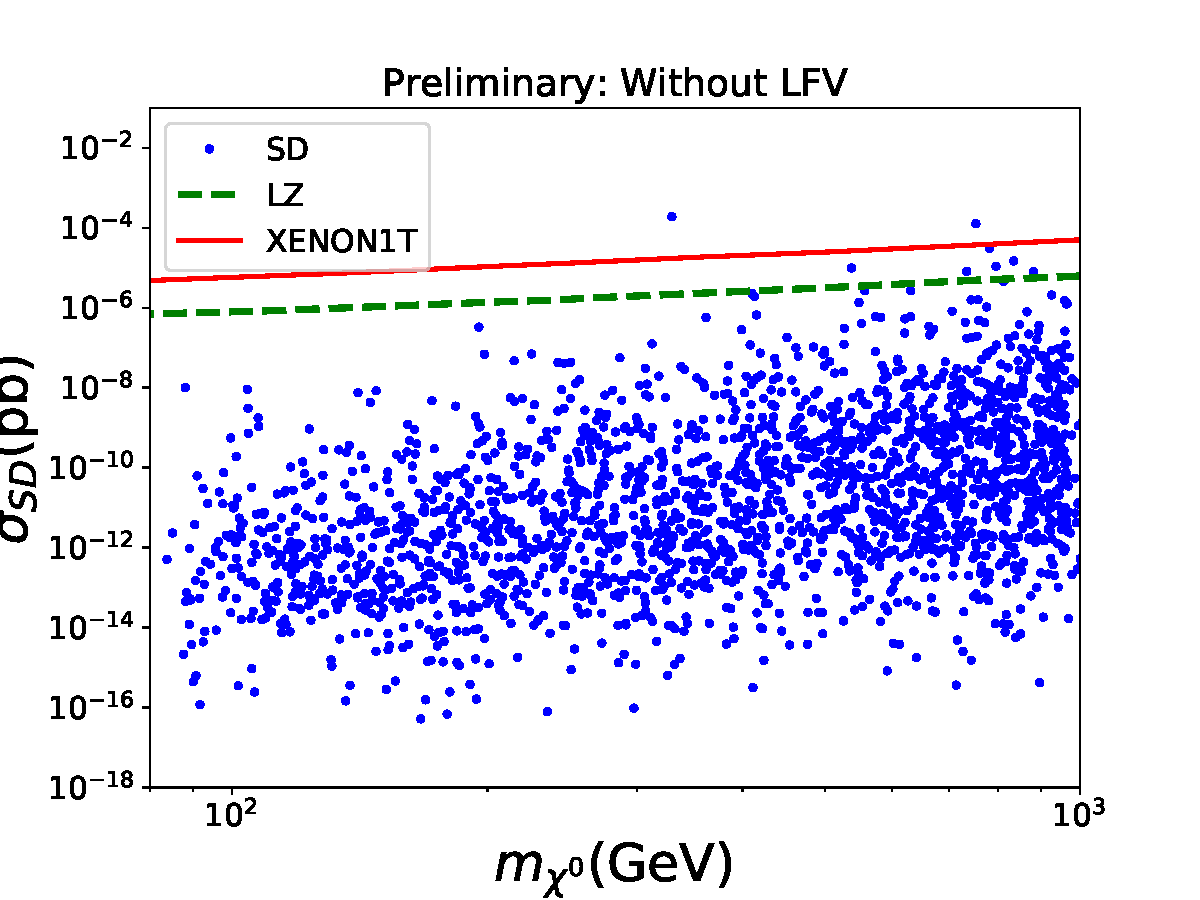
\includegraphics[scale=0.5]{sigmaSD_with_neutrino_physics}
\caption{ SD cross-section  in comparison to current and future direct detection limits.  
%We show the IceCube~\cite{2013PhRvL.110m1302A} limits in the $W^+W^-$ channel (black solid line) from null observations of the sun, and the constraints from LUX~\cite{Akerib:2016lao} (yellow solid lines) limits as well as the LZ and XENON1T sensitivity~\cite{Cushman:2013zza}(red and green dashed line)
}
\label{fig:SD-scan}
\end{center}
\end{figure}
%








\subsection{Gamma-ray signal: DM annihilation into two photons}
\label{sec:gamma-ray}
  
In general, the DM annihilation into photons is a loop process given for multiples topologies. 
It is an interesting process because it would produce a monoenergetic spectral line that would be a strong indication of the existence of the DM. We know that this line-like spectrum is so difficult to explain using the known astrophysical objects in the universe, and for that reason, its finding would be a clear hint of the DM.
     
In this model, the DM could annihilate into two photons ($\chi_1^0\chi_1^0\rightarrow\gamma\gamma$) and into a photon and a one $Z$ gauge boson ($\chi_1^0\chi_1^0\rightarrow\gamma Z$). 
However, in this work, we only compute the amplitude for the former process because we suspect that it is dominant one, the last is off to the scope of this work.
%
Following the general expression given in the ref.~\cite{Garcia-Cely:2016hsk} we computed the general amplitude for the $\chi_1^0\chi_1^0\rightarrow\gamma\gamma$ process. 
Also, we used \texttt{FeynArts}~\cite{Hahn:2000kx} and \texttt{FormCalc} to reduce the tensor loop integrals to scalar Passarino-Veltman functions~\cite{Passarino:1978jh}. Finally, we used \texttt{Package-X}~\cite{Patel:2015tea} to compute the amplitude of this process and to do a cross-check with the general algorithm implemented in~\cite{Garcia-Cely:2016hsk}.
%
The cross-section for this process is given by
%
\begin{align}
\label{eq:sigmav-gg}
\sigma v (\chi^0\chi^0\rightarrow\gamma\gamma) &= \dfrac{|\mathcal{B}|^2}{32\pi m_{\chi^0}^2}\,,
\end{align}
%
where the $\mathcal{B}$ factor is a scalar function. It is given in the Appendix~\ref{app:B-factor}, eq.~\ref{eq:B}, where it was written in such a way that we factorized the gauge invariant contribution in order to see the impact of the different parameters of this model.
Even more, in the Appendix~\ref{app:B-factor} we show that this general expression reproduces some known limits. 
For instance, in the limit of singlet fermion DM, which is, $\alpha =\pi/2$ and $Y_{\Omega}=0$, the eq.~\ref{eq:B} reproduces the amplitude of the original scotogenic model~\cite{Garny:2015wea,Garcia-Cely:2016hsk} as we show in sec.~\ref{sec:pure-singlet-sigmagg}.
In the same way, in the limit of pure triplet DM, that is $Y_{\Omega}=Y_{N}^{\alpha}=Y_{\Sigma}^{\alpha}=v_{\Omega}=0$, $\alpha =0^{\circ}$ and $m=M_{\Sigma}$,  the eq.~\ref{eq:B} reproduces the results obtained in the high mass region for minimal DM model~\cite{Cirelli:2005uq} as we show in sec.~\ref{sec:pure-triplet-sigmagg}.
After doing this check for those two known limits, we disagree with the ref.~\cite{Choubey:2017yyn}. This contribution cannot be extracted from a super-symmetry limit, because that case does not have a pure triplet scalar $\Omega$.

In Fig.~\ref{fig:sigmavgg} we show the DM annihilation into two photons for the scan done in sec.~\ref{sec:full-scan}. We only show the points which are in agreement with the LFV processes described in sec.~\ref{sec:LFV}, neutrino physics~\cite{deSalas:2017kay} and the relic density of DM via the freeze-out mechanism~\cite{Aghanim:2018eyx}.
We also show the current bounds of the Fermi-LAT~\cite{Ackermann:2015lka} collaboration for observation of the Milky Way halo in the low mass region $\sim (200\,\text{MeV}-500\,\text{GeV})$ and the HESS~\cite{Abdallah:2018qtu} bounds for the high mass region $\sim (300\,\text{GeV}-70\,\text{TeV})$.
After improving our scan as much as possible, we realize that all the points always fall under the Fermi-LAT bound in the low mass region. On the other hand, in the high mass region the model reaches the current bound of HESS, however, for those points, the DM is a pure fermion triplet and those points are excluded by the Sommerfeld enhancement~\cite{}.
 
%
\begin{figure}
\begin{center}
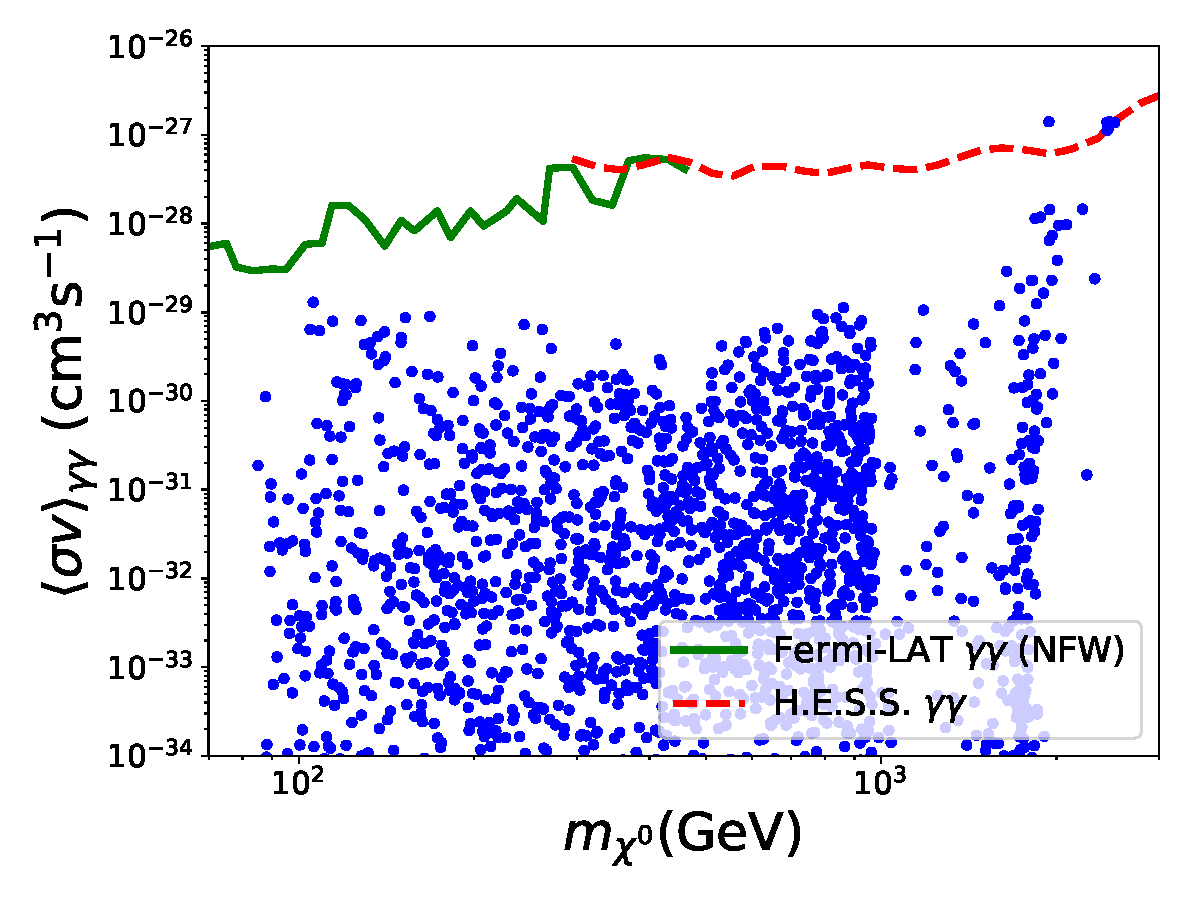
\includegraphics[scale=0.5]{sigmavgg_with_neutrino_physics}
\caption{DM annihilation into two photons in the singlet-triplet scotogenic model. The continues(dashed) line represent the current bound of Fermi-LAT(HESS) collaboration for DM annihilation into two photons in the Milky Way Galaxy.}
\label{fig:sigmavgg}
\end{center}
\end{figure}
%
 
 






 
 
 
 
 
 

\section{Conclusions}
\label{sec:conclusions}

In this work we ...


         

 

\section{Acknowledgments}
We would like to thank ...

\appendix

\section{General $\mathcal{B}$ factor in this model}
\label{app:B-factor}

We factorized the $\mathcal{B}$ factor in gauge invariant terms in order to get clarity in the expression
%
\begin{align}
\label{eq:B}
\mathcal{B} &=
\frac{ \sqrt{2} \alpha  m^2 \sin ^2(\alpha ){\color{red}Y_{\Omega }^2} (\sin (\delta )+\cos (\delta ))^2}{\pi }
\bigg[
\frac{M_{H^{\pm }}^2 C_0\left(0,-m^2,m^2;M_{H^{\pm }}^2,M_{H^{\pm }}^2,M_{\Sigma }^2\right)}{M_{H^{\pm }}^2-M_{\Sigma }^2}\nonumber\\
&-\frac{M_{\Sigma } \left(-2 m M_{H^{\pm }}^2-M_{\Sigma } M_{H^{\pm }}^2+m^2 M_{\Sigma }+2 m
   M_{\Sigma }^2+M_{\Sigma }^3\right) C_0\left(0,-m^2,m^2;M_{\Sigma }^2,M_{\Sigma }^2,M_{H^{\pm }}^2\right)}{\left(M_{H^{\pm }}^2-M_{\Sigma }^2\right) \left(M_{H^{\pm }}^2+m^2-M_{\Sigma }^2\right)}\nonumber\\
&+\frac{2 M_{\Sigma }
   \left(m+M_{\Sigma }\right) C_0\left(0,0,4 m^2;M_{\Sigma }^2,M_{\Sigma }^2,M_{\Sigma }^2\right)}{-M_{H^{\pm }}^2-m^2+M_{\Sigma }^2}
\bigg]\nonumber\\
&+
\frac{\alpha  m^2 \sin (\alpha ) \cos (\alpha ) {\color{red}Y_N^{\alpha } Y_{\Sigma }^{\alpha }}}{\pi }
\bigg[
-\frac{m_{\eta }^2 C_0\left(0,-m^2,m^2;m_{\eta }^2,m_{\eta }^2,m_{e_i}^2\right)}{m_{\eta }^2-m_{e_i}^2}\nonumber\\
&+ \frac{m_{e_i}^2 \left(m_{e_i}^2+m^2-m_{\eta }^2\right) C_0\left(0,-m^2,m^2;m_{e_i}^2,m_{e_i}^2,m_{\eta
   }^2\right)}{\left(m_{\eta }^2-m_{e_i}^2\right) \left(-m_{e_i}^2+m^2+m_{\eta }^2\right)}+\frac{2 m_{e_i}^2 C_0\left(0,0,4 m^2;m_{e_i}^2,m_{e_i}^2,m_{e_i}^2\right)}{-m_{e_i}^2+m^2+m_{\eta }^2}
\bigg]\nonumber\\
&+
\frac{\alpha  m^2 \cos ^2(\alpha ) {\color{red}(Y_{\Sigma }^{\alpha })^2}}{2\sqrt{2} \pi }
\bigg[
\frac{m_{\eta }^2 C_0\left(0,-m^2,m^2;m_{\eta }^2,m_{\eta }^2,m_{e_i}^2\right)}{m_{\eta }^2-m_{e_i}^2}\nonumber\\
&-\frac{m_{e_i}^2 \left(m_{e_i}^2+m^2-m_{\eta }^2\right) C_0\left(0,-m^2,m^2;m_{e_i}^2,m_{e_i}^2,m_{\eta
   }^2\right)}{\left(m_{\eta }^2-m_{e_i}^2\right) \left(-m_{e_i}^2+m^2+m_{\eta }^2\right)}-\frac{2 m_{e_i}^2 C_0\left(0,0,4 m^2;m_{e_i}^2,m_{e_i}^2,m_{e_i}^2\right)}{-m_{e_i}^2+m^2+m_{\eta }^2}
\bigg]\nonumber\\
&+
\frac{\sqrt{2} \alpha  m^2 \sin ^2(\alpha ) {\color{red}(Y_N^{\alpha })^2}}{2\pi }
\bigg[
\frac{m_{\eta }^2 C_0\left(0,-m^2,m^2;m_{\eta }^2,m_{\eta }^2,m_{e_i}^2\right)}{m_{\eta }^2-m_{e_i}^2}\nonumber\\
&-\frac{m_{e_i}^2 \left(m_{e_i}^2+m^2-m_{\eta }^2\right) C_0\left(0,-m^2,m^2;m_{e_i}^2,m_{e_i}^2,m_{\eta
   }^2\right)}{\left(m_{\eta }^2-m_{e_i}^2\right) \left(-m_{e_i}^2+m^2+m_{\eta }^2\right)}-\frac{2 m_{e_i}^2 C_0\left(0,0,4 m^2;m_{e_i}^2,m_{e_i}^2,m_{e_i}^2\right)}{-m_{e_i}^2+m^2+m_{\eta }^2}
\bigg]\nonumber\\
&-
\frac{8 \sqrt{2} \alpha  m^2 \cos ^2(\alpha ) M_W^2}{\pi  \left(M_{\Sigma }^2-M_W^2\right) \left(4 v_{\Omega }^2+v_{\phi }^2\right) \left(m^2-M_{\Sigma }^2+M_W^2\right) \left(m^2+M_{\Sigma }^2-M_W^2\right)}\nonumber\\
&
\bigg[
4 \left(m^2-M_W^2\right) \left(M_{\Sigma }^2-M_W^2\right) \left(m^2-M_{\Sigma }^2+M_W^2\right) C_0\left(0,0,4 m^2;M_W^2,M_W^2,M_W^2\right)\nonumber\\
&+2 M_{\Sigma } \left(2 m-M_{\Sigma }\right) \left(M_{\Sigma }^2-M_W^2\right)
   \left(m^2+M_{\Sigma }^2-M_W^2\right) C_0\left(0,0,4 m^2;M_{\Sigma }^2,M_{\Sigma }^2,M_{\Sigma }^2\right)\nonumber\\
   &-\left(m^2-M_{\Sigma }^2+M_W^2\right) \left(-M_W^2 \left(m^2+M_{\Sigma }^2\right)-4 m M_{\Sigma }
   \left(m^2+M_{\Sigma }^2-M_W^2\right)+4 M_{\Sigma }^4+M_W^4\right)\nonumber\\
   & C_0\left(0,-m^2,m^2;M_W^2,M_W^2,M_{\Sigma }^2\right)-M_{\Sigma } \left(m^2+M_{\Sigma }^2-M_W^2\right) \left(4 m^3-3 m^2 M_{\Sigma }+M_{\Sigma
   }^3-M_{\Sigma } M_W^2\right)\nonumber\\
   & C_0\left(0,-m^2,m^2;M_{\Sigma }^2,M_{\Sigma }^2,M_W^2\right)
\bigg]
\end{align}

\subsection{Pure singlet DM (Scotogenic limit)}
\label{sec:pure-singlet-sigmagg}

The $\mathcal{B}$ factor in this case can be obtained from the eq.~\ref{eq:B} taken $\alpha =\pi/2$, $Y_{\Omega}=0$. In this limit we have
%
\begin{align}
\mathcal{B} &=
\frac{\alpha  m^2 (Y_N^{\alpha })^2}{\sqrt{2} \pi }\bigg[
\frac{m_{\eta }^2 C_0\left(0,-m^2,m^2;m_{\eta }^2,m_{\eta }^2,m_{e_i}^2\right)}{m_{\eta }^2-m_{e_i}^2}\nonumber\\
&-\frac{m_{e_i}^2 \left(m_{e_i}^2+m^2-m_{\eta }^2\right) C_0\left(0,-m^2,m^2;m_{e_i}^2,m_{e_i}^2,m_{\eta
   }^2\right)}{\left(m_{\eta }^2-m_{e_i}^2\right) \left(-m_{e_i}^2+m^2+m_{\eta }^2\right)}-\frac{2 m_{e_i}^2 C_0\left(0,0,4 m^2;m_{e_i}^2,m_{e_i}^2,m_{e_i}^2\right)}{-m_{e_i}^2+m^2+m_{\eta }^2}\bigg]\,.
\end{align}
%
In the limit of $m\gg m_{e_i}$, i.e., when the DM mass is bigger than  standard model lepton masses, this expression gives (we used \texttt{PackageX}~\cite{Patel:2015tea})
%
\begin{align}
\mathcal{B} &=
\dfrac{\alpha(Y_N^{\alpha })^2}{2\sqrt{2}\pi}
\left[\text{Li}_2\left(\dfrac{m^2}{m_{\eta}^2}\right)-\text{Li}_2\left(-\dfrac{m^2}{m_{\eta}^2}\right)\right]\,.
\end{align}
Therefore, using the eq.~\ref{eq:sigmav-gg}, we have
%
\begin{align}
\sigma v = \dfrac{|\mathcal{B}|^2}{32\pi m^2}=\dfrac{\alpha^2(Y_N^{\alpha })^4}{256\pi^3}\left[\text{Li}_2\left(\dfrac{m^2}{m_{\eta}^2}\right)-\text{Li}_2\left(-\dfrac{m^2}{m_{\eta}^2}\right)\right]^2\,,
\end{align}
in agreement with the ref.~\cite{Garny:2015wea}.



\subsection{Pure triplet DM (Minimal DM limit)}
\label{sec:pure-triplet-sigmagg}
The $\mathcal{B}$ factor in this case can be obtained from the eq.~\ref{eq:B} taken $Y_{\Omega}=Y_{N}^{\alpha}=Y_{\Sigma}^{\alpha}=v_{\Omega}=0$, $\alpha =0$ and $m=M_{\Sigma}$. In this limit we have
%
\begin{align}
\mathcal{B} &=
\frac{8 \sqrt{2} \alpha ^2 m^2}{\sin(\theta_W)^2}
\bigg[
\frac{m^2 \left(M_W^2-2 m^2\right) C_0\left(0,-m^2,m^2;m^2,m^2,M_W^2\right)}{M_W^2 \left(M_W^2-m^2\right)}-\frac{2 m^2 C_0\left(0,0,4 m^2;m^2,m^2,m^2\right)}{M_W^2}\nonumber\\
&-\frac{4 \left(M_W^2-m^2\right) C_0\left(0,0,4
   m^2;M_W^2,M_W^2,M_W^2\right)}{M_W^2-2 m^2}\nonumber\\
   &+\frac{\left(-4 m^4+2 m^2 M_W^2+M_W^4\right) C_0\left(0,-m^2,m^2;M_W^2,M_W^2,m^2\right)}{2 m^4-3 m^2 M_W^2+M_W^4}
\bigg]\,.
\end{align}
In the limit of $m\gg M_W$ we get (we used \texttt{PackageX}~\cite{Patel:2015tea}) 
\begin{align}
\mathcal{B} 
&\approx \frac{\sqrt{2} \pi  \alpha ^2 m \left(-8 m^2+\pi  m M_W+4 M_W^2\right) \csc ^2\left(\theta _W\right)}{M_W^3-m^2 M_W}\,,
\end{align}
and therefore, using the eq.~\ref{eq:sigmav-gg}, we have get that 
\begin{align}
\sigma v = \dfrac{|\mathcal{B}|^2}{32\pi m^2}\approx
\frac{4 \pi  \alpha ^4 \left(\theta _W\right)}{M_W^2 \sin(\theta_W)^4}\,,
\end{align}
in agreement with the ref.~\cite{Cirelli:2005uq}.









\bibliographystyle{jhep}
\bibliography{references}



\end{document}

